\documentclass[12pt, twoside]{article}
\usepackage[left=2.5cm,right=2cm,top=2cm,bottom=2cm]{geometry}

\usepackage{lastpage}
\usepackage{fancyhdr}
\pagestyle{fancy}
\renewcommand{\headrulewidth}{0.4pt}
\renewcommand{\footrulewidth}{0.4pt}
\renewcommand{\sectionmark}[1]{ \markright{#1}{} }
\lhead{Cyril NOVEL (cbn13)}\chead{}\rhead{\textit{ \nouppercase{\rightmark}}}
\lfoot{}\cfoot{\thepage\ of \pageref{LastPage}}\rfoot{}

\setlength{\headheight}{15pt}

\usepackage[english]{babel}
\usepackage[utf8]{inputenc}
\usepackage{amsmath}
\usepackage{graphicx}
%\usepackage{algpseudocode}
\usepackage{algorithm}
\usepackage{amsthm}
\usepackage{amssymb}
\usepackage{mathtools}
\usepackage{commath}
\usepackage{stmaryrd}
\usepackage{url}
\usepackage{caption}
\usepackage{subcaption}
\usepackage{hyperref}
\usepackage[noend]{algpseudocode}
\usepackage{listings}
\usepackage[usenames,dvipsnames,svgnames,table]{xcolor} % for setting colors
\usepackage{courier}

\let\oldsection\section
\def\section{\cleardoublepage\oldsection}

\renewcommand*\lstlistingname{Code}
% set the default code style
\lstset{
    frame=tb, % draw a frame at the top and bottom of the code block
    tabsize=2, % tab space width
    showstringspaces=false, % don't mark spaces in strings
    numbers=left, % display line numbers on the left
    commentstyle=\color{gray}, % comment color
    keywordstyle=\color{blue}, % keyword color
    stringstyle=\color{red}, % string color
    basicstyle=\footnotesize\ttfamily
}

\hypersetup{
  colorlinks=true,
  citecolor=black,
  urlcolor=Cerulean,
  linkcolor=PineGreen,
}

\title{OFusion\\
\large{CO542 Individual Project}}

\author{Cyril NOVEL}

\date{\today}

\begin{document}

\begin{titlepage}
\begin{center}

\includegraphics[width=0.15\textwidth]{logo.jpeg}~\\[1cm]

\textsc{\LARGE Imperial College of London}\\[0.5cm]

\textsc{\Large Department of Computing}\\[1.5cm]

% Title
\rule{\textwidth}{.4pt}
{ \huge \bfseries Kinect and Oculus Rift: a new kind of augmented reality device \\[0.4cm] }

\rule{\textwidth}{.4pt}\\[1.5cm]

% Author and supervisor
\begin{minipage}{0.4\textwidth}
\begin{flushleft} \large
\emph{Author:}\\
Cyril \textsc{Novel}
\end{flushleft}
\end{minipage}
\begin{minipage}{0.4\textwidth}
\begin{flushright} \large
\emph{Supervisor:} \\
Prof. Andrew \textsc{Davison}
\end{flushright}
\end{minipage}

\vfill
{Submitted in partial fulfilment of the requirements for the MSc Degree in Computing Specialism -- Visual Information Processing -- of Imperial College London}\\[0.4cm]
{\large \today}
\end{center}
\end{titlepage}

\newpage
\begin{abstract}
The Oculus Rift is a device capable of displaying 3D information on the whole field of view of the user. The Kinect is a RGBD camera, capable of computing a depthmap of the scene it is looking at. In this project, we propose to combine the Oculus Rift and the Kinect to create a new kind of augmented reality device. With the algorithm KinectFusion, we are capable of computing a 3D representation of the surrounding scene and display it into the Rift for the user. To reinforce the immersion, we introduce live color projection on the scene. The Rift and the Kinect are correctly calibrated to provide the best user experience.

We also present an augmented reality application called \textit{magical pen} where the user can freely draw on a surface.
\end{abstract}~\\[5cm]
%\addcontentsline{toc}{section}{Abstract}

\section*{Acknowledgements}
\addcontentsline{toc}{section}{Acknowledgements}
I would like to thank Professor Andrew Davison for his help and indications throughout this project. Thank you to Steven Lovegrove, who helped me on the crucial point of Lens distortion for Rift rendering.
\newpage

\tableofcontents

\newpage

\section*{Introduction}
\addcontentsline{toc}{section}{Introduction}
Augmented reality is an active field in Computer Science and Computer Vision, with the multiplication of portable devices with high perfomance CPU and GPU. Multiples devices are providing an augmented reality experience. The Nintendo 3DS has a dedicated game with augmented reality cards, applications can be downloaded on smartphones. The Google Glass works like a small Head Up Display for the user, similar to what can be seen in some videogames. The Project Tango phone and tablet comes with built-in augmented reality applications. However, none of these devices are capable of displaying information for the entire field of view of the user. The smartphone or tablet size is small compared to the size of the field of view. The Google Glass encounters the same problem: there is no possible overlay of the reality.

By using a virtual reality headset, such as the Oculus Rift, we cover the entire field of view of the user. Using an appropriate sensor, we can understand the scene surrounding the user. Then we can overlay information on the reality for the whole field of view. This creates a new kind of augmented reality device. Applications are infinite: the road to follow can be directly highlighted in a GPS application; you can play a virtual game in your living room with the game understanding the geometry of your living room -- making each game unique since you can move objects; a medical application can highlight organs during an operation and also provide an HUD with useful information. Possibilities are countless.

During this project, we created a device fusionning an Oculus Rift and a Kinect to create a new kind of augmented reality device. The Kinect captures the surrounding scene. It is then rendered in 3D in the Oculus Rift with real-time color information. Thus the user can evolve just like in real life. An augmented reality application has been integrated. Using a \textit{magical pen}, it is possible to draw virtually on a surface.
\newpage

\section{Hardware review}
\subsection{Virtual reality headsets}
A virtual reality headset is a device capable of displaying 3D scenes to the user wearing the headset. It is made of screen and two lenses, with the left part of the screen showing the image for the left eye and the right part for the right eye.

Virtual reality headsets have been fancied a long-time and are finally becoming reality. The Oculus Rift is the first affordable headset to encounter a commercial success. Previously, Nintendo tried to sell a virtual reality headset called the Virtual Boy. It was a failure since its use caused terrible headaches to the players and only 5 shades of red were available.

In the following sections, we will present some virtual reality headsets and highlight their differences.

\subsubsection{Oculus Rift and Sony Morpheus}
The Oculus Rift is developped by Oculus VR \cite{Oculus}. It is the first virtual headset targeting the mass market, and therefore has an aggressive price -- the first development kit costs 300\$, 350\$ for the second one.

The Oculus uses an LCD screen for displaying the image. In the first development kit, the resolution of the screen was 1280x800, leading to an effective 640x800 per eye. One part of the screen displays the image for one eye, the other part displays the image for the other eye. The Rift uses lenses to distort the image on the screen, so that it fits the actual field of view of the human eye. The field of view of the Rift is 90 degrees horizontally. Figure~\ref{fig:oculusback} shows the back of the Oculus Rift.

A gyroscope, an accelerometer and a magnetometer are combined in the headset in order to track the user's head movements. The first development kit is however unable to detect translation movement.

\begin{figure}[h]
  \centering
  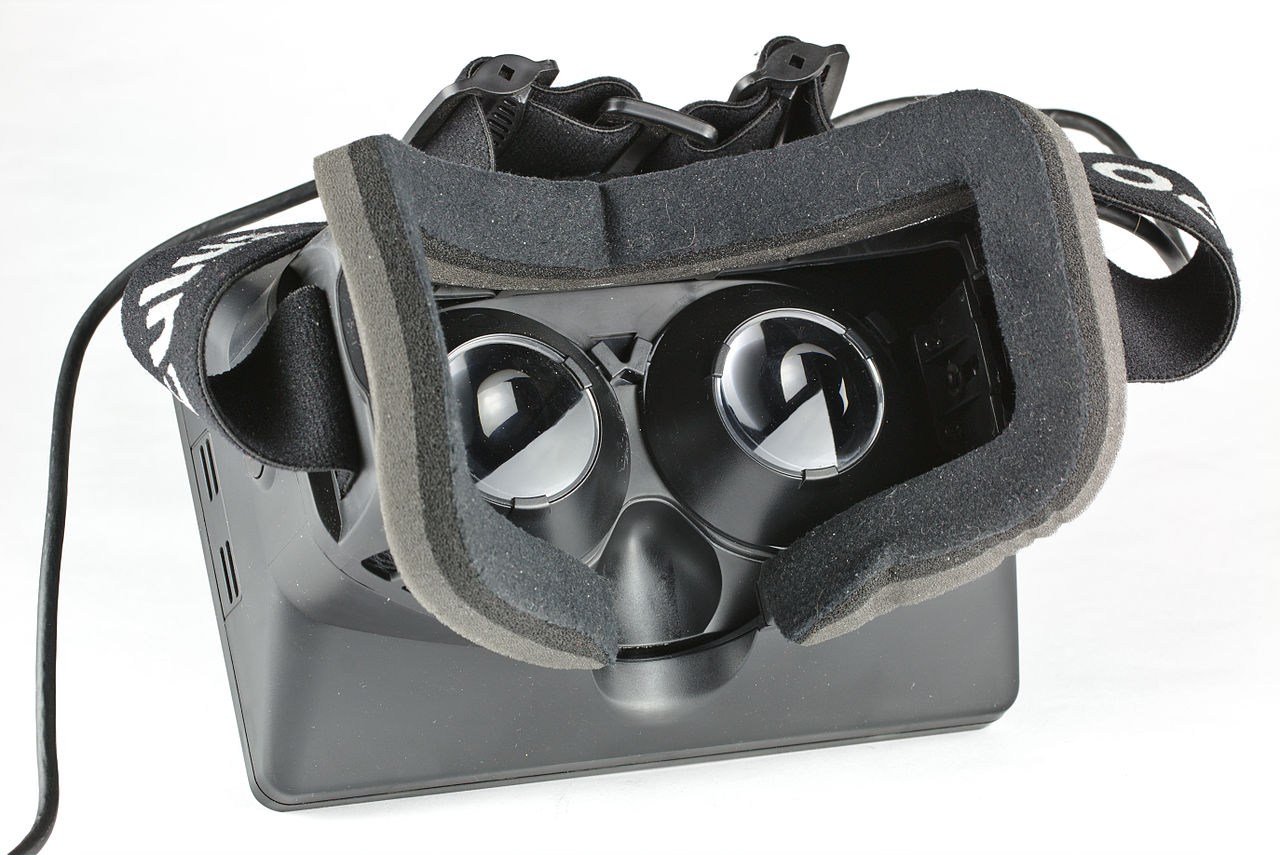
\includegraphics[scale=0.2]{OculusBack.jpg}
  \caption{\label{fig:oculusback} The Oculus Rift\protect\footnotemark}
\end{figure}
\footnotetext{Photo CC-BY 3.0 by Sebastian Stabinger}

The major drawback of the Rift is the resolution of the screen. The screen-door effect is predominant and prevent a total immersion in the displayed scene. The second version of the Development Kit comes with a resolution of 960x1080 per eye, decreasing this effect. This next version comes also with a camera, tracking the movement of the head, in order to detect translation in addition to rotation.

The success of the Oculus Rift leads other companies to develop similar devices. Sony presented few months ago the project Morpheus \cite{Morpheus} -- shown in Figure~\ref{fig:morpheus}, highly similar to the Oculus Rift.

\begin{figure}[h]
  \centering
  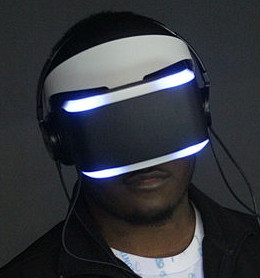
\includegraphics[scale=0.5]{Morpheus.jpg}
  \caption{\label{fig:morpheus} Sony Morpheus\protect\footnotemark}
\end{figure}
\footnotetext{Photo CC-BY 2.0 by GDC Official}

Sony Morpheus uses a comparable technology to the Oculus Rift. The most noticeable difference is that Morpheus has tracking technology all around it, whereas Oculus Rift only has tracking captors on the front and on the sides of the display.

\subsubsection{Google Cardboard and Samsung Gear VR}
During the Google I/O 2014, Google introduced the Cardboard Project. The idea is to use a smartphone as the screen for the headset and create the headset from a cardboard. Google presented the project as a Do-It-Yourself headset, acknowledging that the most difficult part was purchasing the lenses. The design files are available online and some online stores sell and ship the set for 25\$.

\begin{figure}[h]
  \centering
  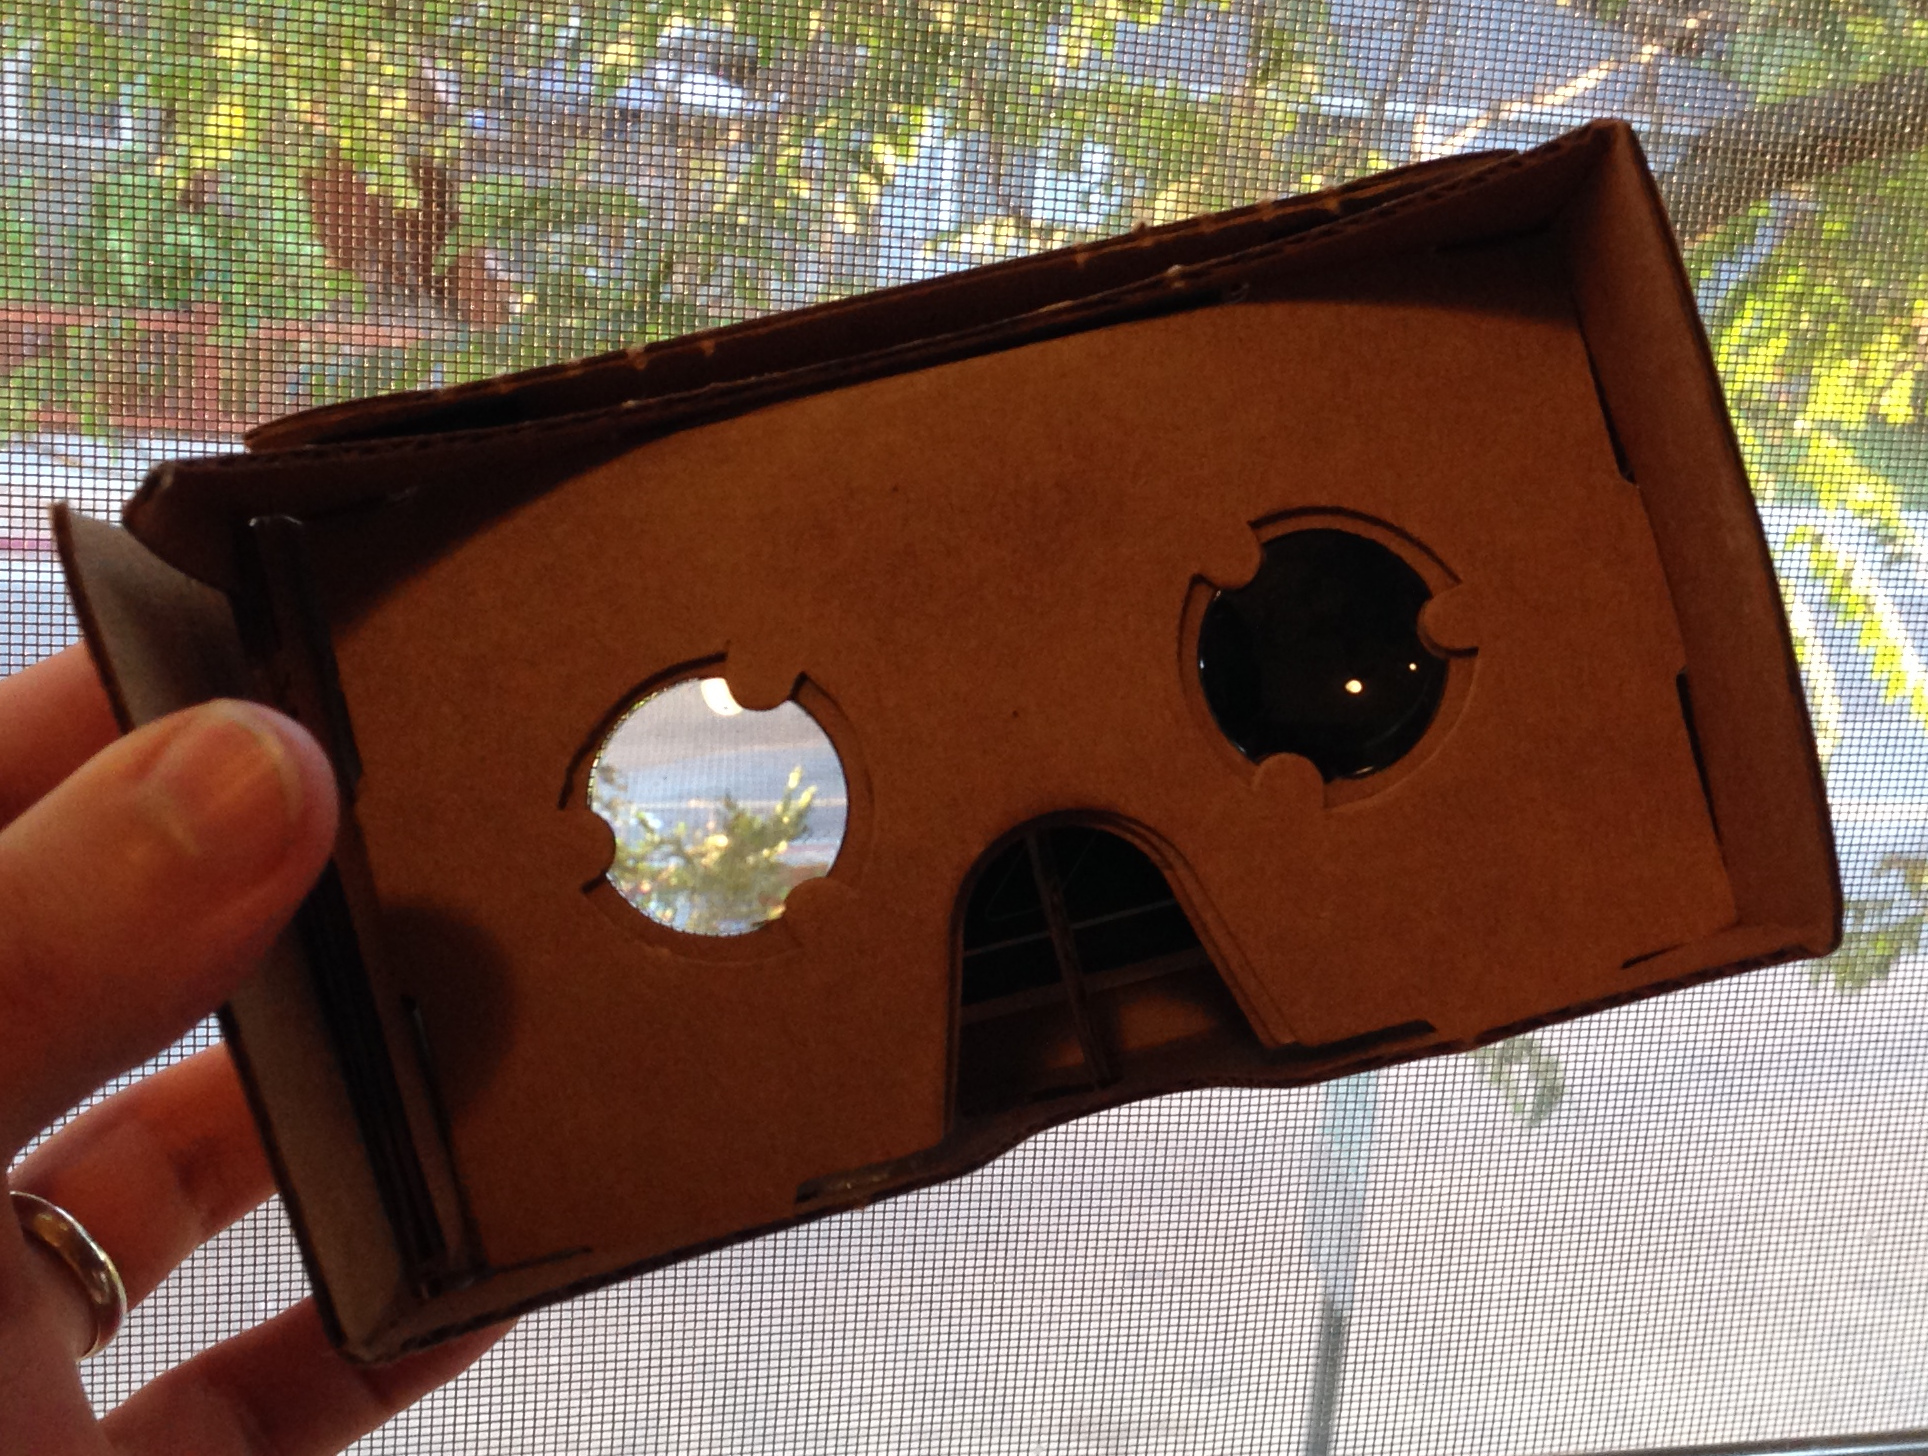
\includegraphics[scale=0.1]{GoogleCardboard.jpg}
  \caption{\label{fig:cardboard} The Google Cardboard project\protect\footnotemark}
\end{figure}
\footnotetext{Photo BY-SA 3.0 by Runner1928}

The advantage of Google Carboard is that it uses the sensors in the smartphone for the head positionning. Every recent smartphone is equiped with a gyroscope and a magnetometer, so the head tracking is easy to achieve.

Samsung is developping a similar headset called Gear VR. Reveal during the IFA 2014, the Gear VR is an headset where the user can place a Galaxy Note 4 as the main screen. The sensors from the Note are assisted by sensors from the Gear VR. The system offers $1280\times 1440$ pixels for each eye, but does not track the translation movement of the user.

The main advantage of smartphones is the high pixel density of the screen. The LG G3 offers a 538 ppi screen, when the first Oculus Rift development kit has \textit{only} a 216 ppi screen. This high density screen counters the screen door effect.

\subsubsection{Vrvana Totem}
The Totem, developed by Vrvana \cite{Vrvana}, is similar to the Oculus Rift, except that two cameras are embedded on the front of the headset -- see Figure~\ref{fig:tpg}. The idea is that each camera captures the view of one eye.

\begin{figure}[h]
  \centering
  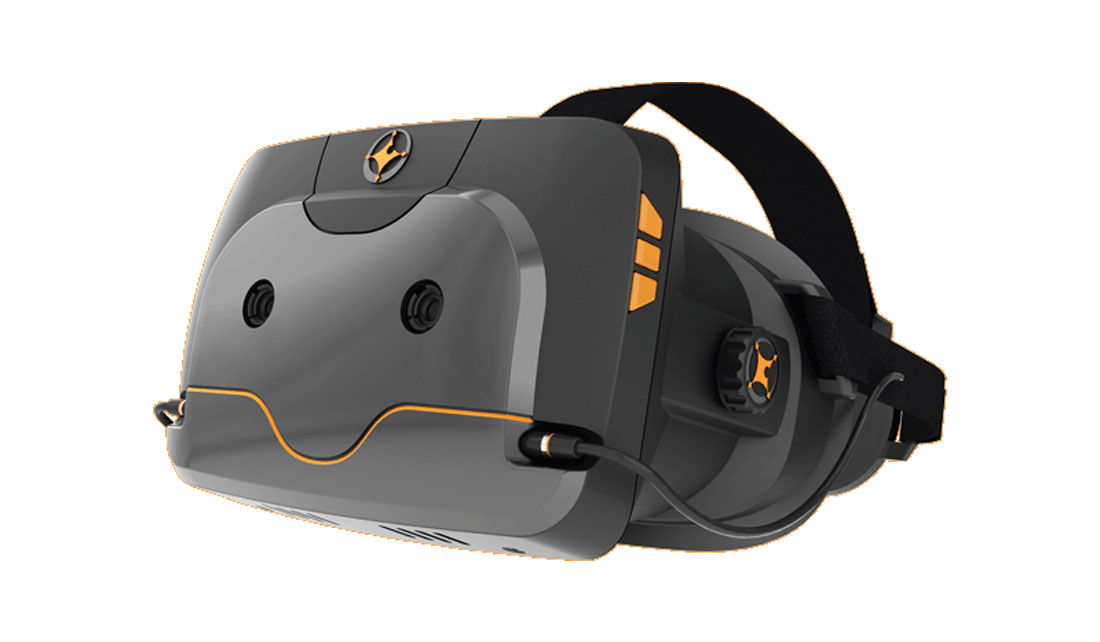
\includegraphics[scale=0.3]{TruePlayerGear.jpg}
  \caption{\label{fig:tpg} The Totem, with two cameras\protect\footnotemark}
\end{figure}
\footnotetext{Photo courtesy of Vrvana}

The lens distorsion is computed directly via the hardware in the headset. The others characteristics are higly similar to the Oculus Rift. The Totem is very interesting thanks to these embedded cameras. We want to achieve a new type of augmented reality. The Totem directly captures what the eyes would see. This guarantees an almost perfect 3D image for the user. However, the 3D reconstruction is more difficult - as seen in section~\ref{subsec:stereocam}.

\subsection{Capturing the scene}
For rendering the scene in a virtual reality headset, we need to capture the scene surrounding the user. We can not just extract features from the scene. We need dense information about the scene in real time in order to create the corresponding 3D surface. In this part we present different devices that can compute a point cloud in real time.

\subsubsection{Structured light scanning}
Structured light scanning is a technique used for computing a depth map from the projection of near IR light patterns on the scene. The device project an IR light pattern on the surface of the room. Depending on the depth of the objects, the pattern is bigger or smaller than the reference pattern. Thus we can infer a depth map by reading the projection of the IR pattern. An exemple of pattern is presented in Figure~\ref{fig:kinectir}.

\begin{figure}[h]
  \centering
  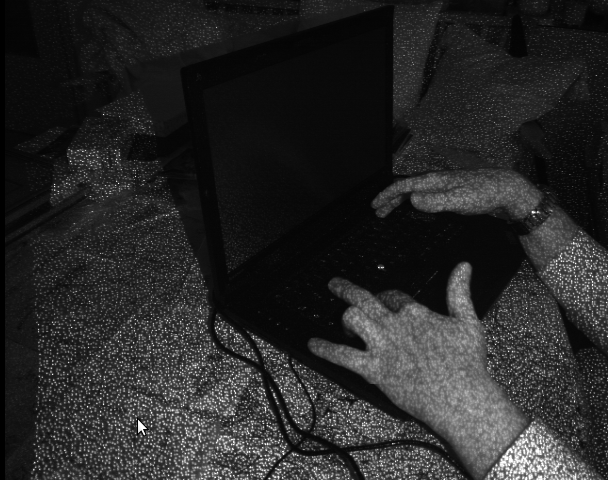
\includegraphics[scale=0.3]{Kinect-ir-image.png}
  \caption{\label{fig:kinectir} Kinect IR pattern\protect\footnotemark}
\end{figure}
\footnotetext{Photo CC BY-SA 3.0 by Kolossos}

This technique is used by the first Kinect -- Figure~\ref{fig:kinect}. The resolution of the depth map is $320*240$ points. Other devices using this technique exist, such as the Asus Xtion or the PrimeSense Capri sensor.

\begin{figure}[h]
  \centering
  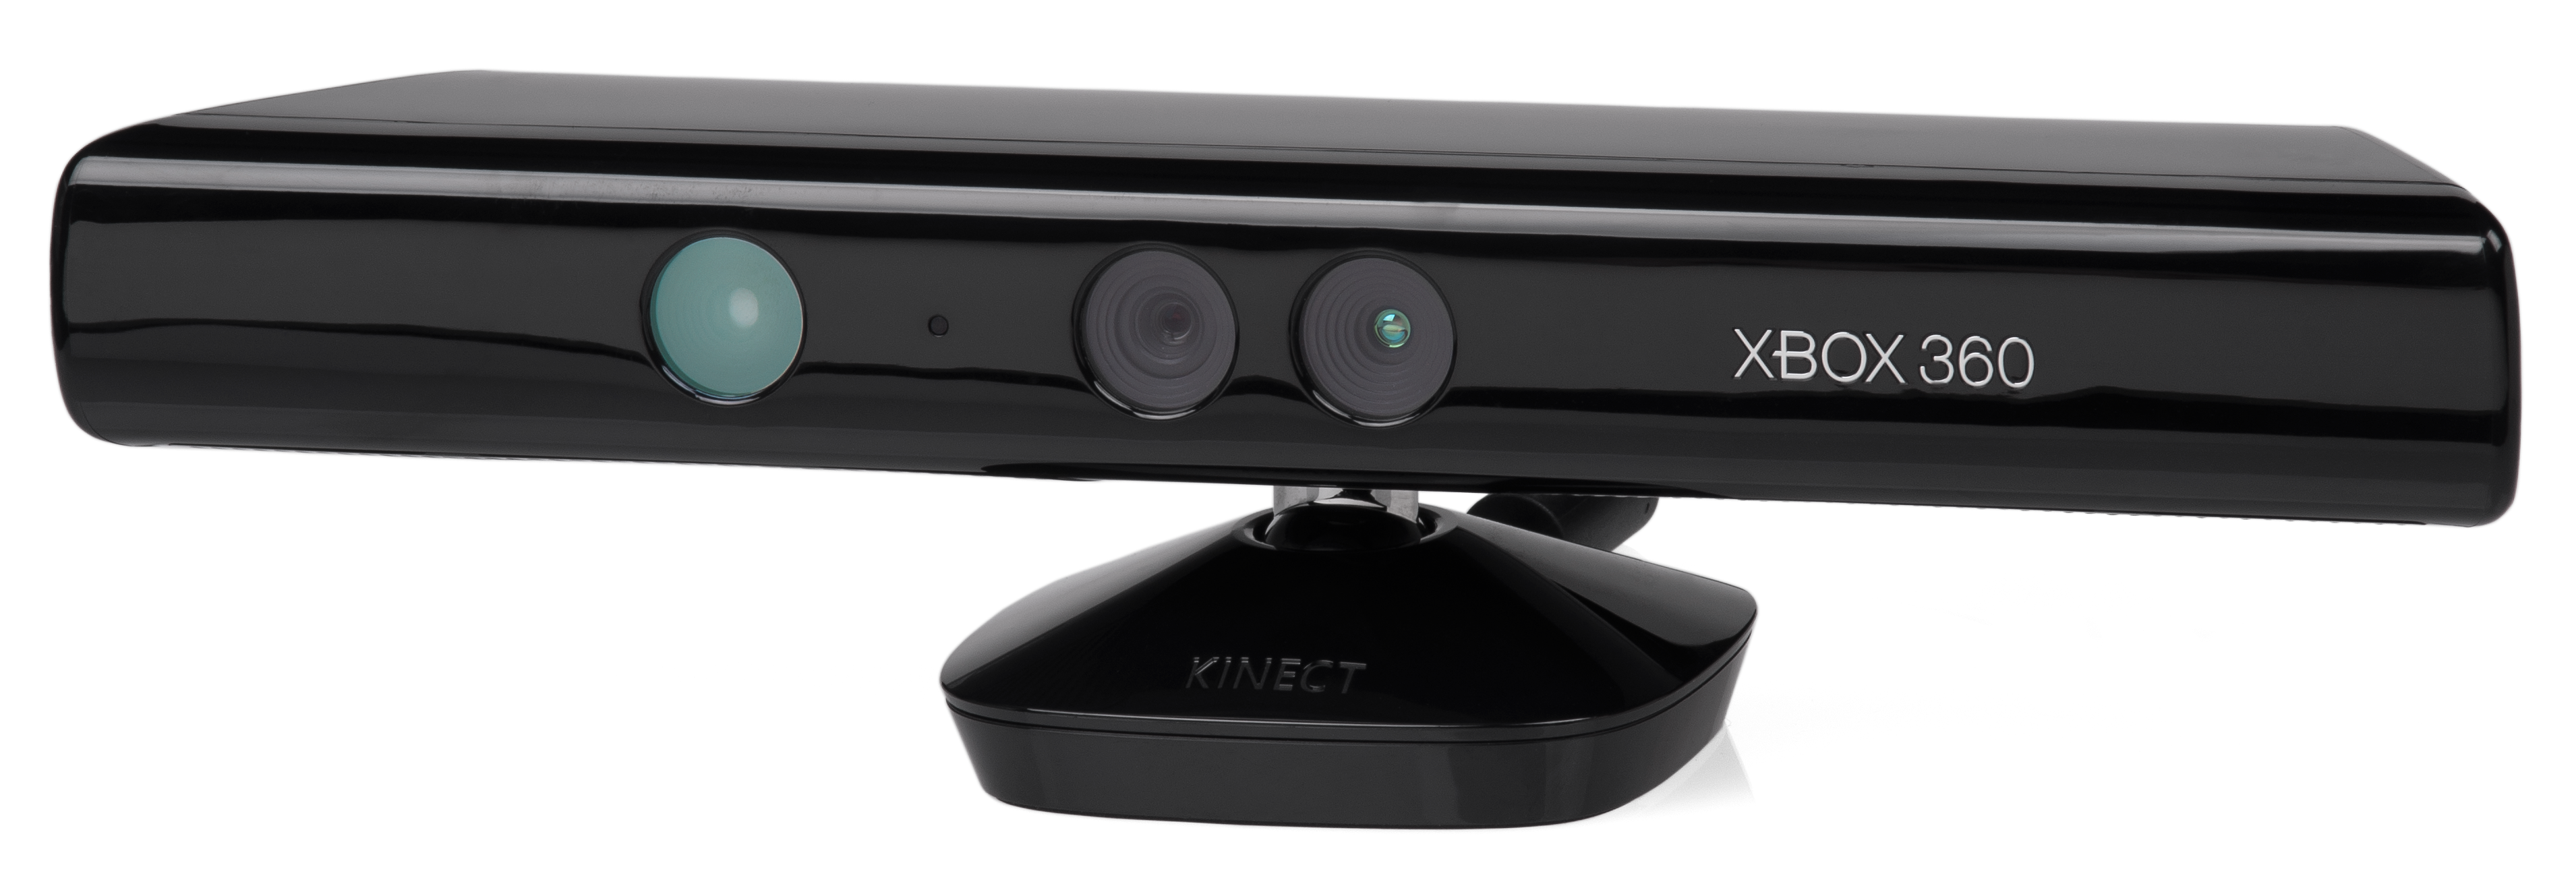
\includegraphics[scale=0.05]{kinect1.png}
  \caption{\label{fig:kinect} First Kinect. From left to right: IR Pattern projector, IR Camera for reading the projected pattern, RGB camera}
\end{figure}

It is now possible to create very small IR light projector and IR light captor. The Capri sensor is ten times smaller than the Kinect sensor and can be easily mounted on a tablet or a virtual reality headset.

However, the use of structured light comes with drawbacks. In very luminous area, the IR light captor can't work because the incoming light is blinding it. Surfaces like TV or computer screen reflect the IR light and so no information can be retrieve from these areas. Finally, the distance between the projector and the captor creates a shadow effect around the object. Very close objects can't be processed since they aren't properly seen by the captor or the sensor. And since the light intensity decreases with the distance, remote objects can't be seen. The computed distance is sometimes wrong for large distances (more than 4 meters). The depth distribution is discrete and coarse for large distance. Beyond four meters, the depth estimation is often considered as unreliable.

\subsubsection{Time of Flight}
A Time of Flight camera is estimating the distance of a point based on the known speed of light. The camera relies on light pulse. The illumination is switched on for a very short time on one point. The light reflects on the object and is gathered by the camera. The delay between the start of the pulse and the gathering by the camera is the time taken by the light to travel twice the distance between the camera and the object. Knowing the speed of light, we can deduce the distance of the point.

Kinect 2 is using a time of flight camera -- Figure~\ref{fig:kinect2}. The resolution is much higher than the first Kinect, since Kinect 2 produces a $512*424$ depth map. The time of flight doesn't suffer from illumination problems, position problems or distance problems. The depth distribution is not coarse in the remote areas, allowing a nice accuracy of the measurements -- see Figure~\ref{fig:depthK2}.

\begin{figure}[h]
  \centering
  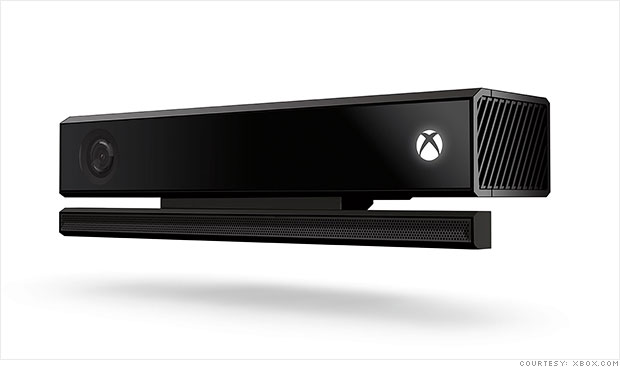
\includegraphics[scale=0.05]{kinect2.jpg}
  \caption{\label{fig:kinect2} Kinect 2}
\end{figure}

\begin{figure}[h]
  \centering
  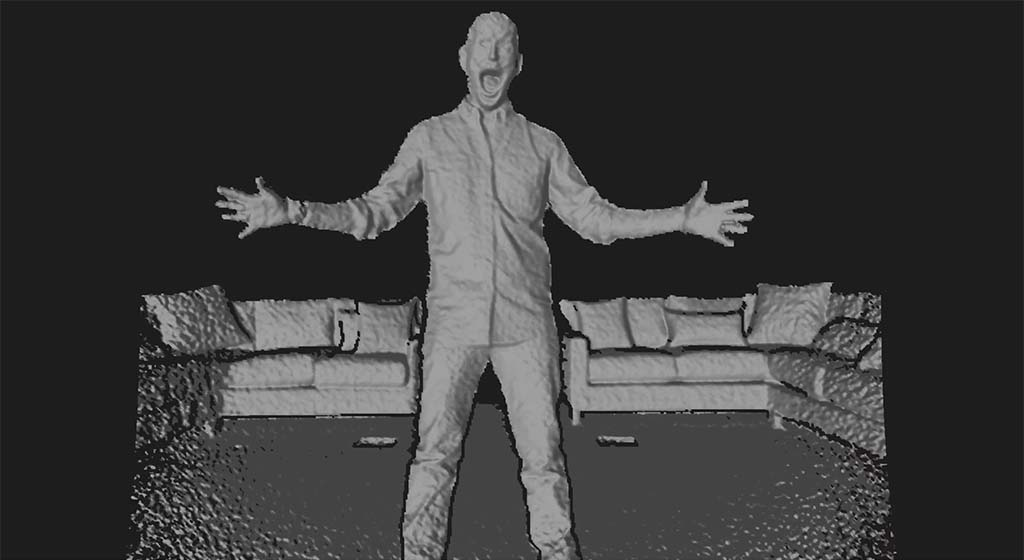
\includegraphics[scale=0.3]{kinect2depth.jpg}
  \caption{\label{fig:depthK2} Depth map with the time of flight camera of the Kinect 2\protect\footnotemark}
\end{figure}
\footnotetext{From the Kinect 2 - Tech Demo footage by Microsoft}

However, Time Of Flight cameras are very expensive, especially for 30Hz processing of the environment. Until recently, real-time TOF cameras had a lower resolution than the Kinect 1. Due to the nature of light reflectivity, the depth estimation is less reliable when the light ray is not perpendicular to the surface. Figure~\ref{fig:depthK2} shows a lot of noise and holes at the extremities of the depth map.

\subsubsection{Stereo camera}
\label{subsec:stereocam}
Stereoscopy uses two or more pictures for finding corresponding features and replace them in 3D space. Given two images of the same object from slightly different points of view, we identify the features that appear on both images. This search is easily performed with the use of Computational Stereo techniques, such as the computation of the epipolar lines. Since we know where the images have been taken relatively to each others, we can compute the depth of the feature. We perform this for every features and we retrieve a point cloud with the approximate same resolution as the images taken.

The chinese company Etron is selling very small devices with two optical captors and a processor for computing the depth map. A resulting depthmap is shown in Figure~\ref{fig:etron}.

\begin{figure}[h]
  \centering
  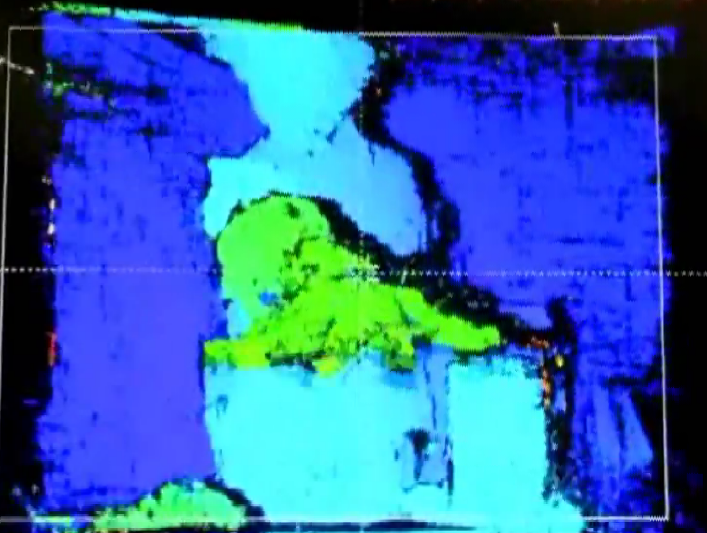
\includegraphics[scale=0.3]{EtronDepth.png}
  \caption{\label{fig:etron} Depth map with two stereo camera}
\end{figure}

Stereo camera system is the cheaper system for retrieving a point cloud. It only requires some calibration and computation, but it is not a very expensive hardware compared to the other two systems.

The computed depth map is unfortunately very noisy. There is a lot of noise when we compute the depth map. Shadow effects can be seen on Figure~\ref{fig:etron}. Moreover it is very difficult to compute a distance for uniform area, since no feature information can be retrieved. We need to extrapolate the distance based  on the surrounding information, but this leads to low fidelity reconstruction of the scene.

\subsection{Similar projects}
The combination of the Oculus Rift with the Kinect has been achieved recently by some researchers.

Thomas Whelan has combined the Oculus Rift and its algorithm Kintinuous \cite{KinRift} -- an extension of KinectFusion algorithm. Kintinuous scans the surrounding scene and computes offline the geometry and the colors of the scene. Then the user puts on the Oculus Rift and the Kinect is set in front of the Rift. The Kinect acts here as the position tracker of the Rift. No live colors are displayed and the user doesn't have any feedback from his body. Because there is no body awareness and no live feedback when the user is moving an object, the experience can be quite disturbing.

Steven Lovegrove has combined the Oculus Rift and KinectFusion \cite{OculusFusion}. This prototype is close to what we are doing in this project. The Kinect simultaneously captures the scene and track the position of the Rift. However, there is no color in this implementation.

\subsection{Conclusion}
Since the success of the Oculus Rift on Kickstarter, multiple companies are creating Virtual Reality headsets. With consummer versions scheduled for 2015, it is very probable that these headsets will encounter a great success. During the same time, huge progress has been made for light weight and cheap scanning devices for capturing the geometry of a scene surrounding the user. Therefore we think it is very probable to see augmented reality applications by combining these two kind of devices in the future.

For our project, we use an Oculus Rift Development Kit 1 with a Kinect for Xbox 360.

\newpage
\section{Theoretical considerations}
\subsection{KinectFusion}
For the reconstruction of the scene and the localization of the user, we use the KinectFusion algorithm. The KinectFusion algorithm achieves real-time dense surface mapping and reconstruction. The algorithm is fully described in \cite{KF1, KF2}. The GPU implementation of KinectFusion allows the real time reconstruction and localization. The algorithm is composed of four main stages:
\begin{enumerate}
\item \textbf{Depth Map conversion} The live depth map is converted into absolute 3D positions and normals in the camera coordinate space;
\item \textbf{Camera tracking} We keep a rigid 6 degrees of freedom transform of the camera. At time $i$, the camera pose is noted $T_i = [R_i|t_i]$ with $R_i$ being a 3x3 rotation matrix and $t_i$ being a 3D translation vector. We use the Iterative Closest Point algorithm for tracking the position and orientation of the camera.
\item \textbf{Volumetric integration} We use a voxel 3D grid to store Truncated Signed Distance Functions that represents the distance to the scene surface.
\item \textbf{Raycasting} The volume is raycasted to render the implicit surface.
\end{enumerate}

Each of this stage is performed in parallel on the GPU using CUDA.

\subsubsection{Depth Map conversion}
The depth map is a 2D array of float. At time $i$, for each pixel $u(x,y)$ we have the corresponding depth $D_i(u)$. The camera matrix is a $4\times 3$ matrix that links a 3D world point to a 2D image point. We are working with homogeneous coordinates, meaning a 2D vector is represented by 3 coordinates and a 3D vector is represented by 4 coordinates. The homogeneous representation makes it easier to compute translation via matrix multiplications.

Given the camera matrix $K$ of the Kinect infrared camera, we can compute the 3D position in the camera coordinate space. For each pixel $u$, a GPU thread computes the 3D position as follow:
$$v_i(u) = D_i(u)K^{-1}[u,1]$$
$[u,1]$ are the homogeneous coordinates of the pixel. $K^{-1}[u,1]$ gives us corresponding 3D point at distance 1 from the camera. The results are saved in a single vertex map $V_i$.

We also compute the corresponding normal map, as it will be useful later for the ICP algorithm. Each normal $n_i(u)$ is computed by a GPU thread using the neighboring reprojected points formula:
$$n_i(u) = (v_i(x+1,y) - v_i(u))\times (v_i(x,y+1) - v_i(u))$$
The normal is then normalized and stored in a single normal map $N_i$.

Given the rigid body transform of the camera $T_i = [R_i|t_i]$, we can convert the vertices and the normals into global coordinates:
$$v_i^g(u) = T_iv_i(u)$$
$$n_i^g(u) = R_in_i(u)$$

\subsubsection{Camera tracking}
Iterative Closest Point algorithm was introduced by \cite{ICP1}. It is a widely studied algorithm for 3D shapes alignement. \cite{ICP2} provides a detailed study of the ICP algorithm. In KinectFusion, ICP is also used for tracking the camera pose of the Kinect, that means its position and its orientation. For each new depth frame captured by the Kinect, the algorithm estimates the 6DOF transform that aligns the vertices and normals of the current frame with those of the previous frame. This gives a relative 6DOF transform. If we apply them together incrementally, we obtain the global camera pose $T_i$.

The first part of the ICP is to find correspondences between the current oriented points set at time $i$ with the previous one at time $i-1$. KinectFusion uses \textit{projective data association}. Given the previous global rigid body transform $T_{i-1}$, each GPU thread projects a point $v_{i-1}$ into camera coordinate space. It then looks up the corresponding point in $V_i$ and in $N_i$ (respectfully the current vertex map and the current normal map). Doing so, we find the corresponding points along the same ray. Next, each thread tests the corresponding points to reject outliers. We compute the euclidean distance between the two global positions and angle between the two corresponding normals. If both of them are within a threshold, the match is validated. A pseudo-code of the algorithm is described in Algorithm~\ref{algo1}. $T_i$ is initialized at $T_{i-1}$ and is updated with an incremental transform at the end of each step of the ICP.

\begin{algorithm}
\caption{Projective point-plane data association}\label{algo1}
\begin{algorithmic}[1]
\For{$\text{each pixel } u \in \text{ depth map } D_i \text{ in parallel}$}
  \If{$D_i(u) > 0$}
  \State $v_i \gets T_{i-1}^{-1}v_{i-1}^g$
  \State $p \gets \text{perspective project vertex of } v_{i-1}$
    \If{$p \in \text{ vertex map } V_i$}
    \State $v \gets T_iV_i(p)$
    \State $n \gets R_iN_i(p)$
      \If{$\left\|v-v_{i-1}^{g}\right\| < \text{ distance threshold and } abs(n\cdot n_{i-1}^{g}) < \text{ normal threshold}$}
      \State point match found
      \EndIf
    \EndIf
  \EndIf
\EndFor
\end{algorithmic}
\end{algorithm}

All the corresponding points are saved into the same set. The output of each ICP iteration is a transformation matrix $T$ that minimizes the point-to-plane metrics, defined as follows:
$$\text{arg min } \sum_{D_i(u)>0} \left\|(Tv_i(u)-v_{i-1}^g(u))\cdot n_{i-1}^g(u) \right\|^2$$

Assuming only an incremental transform occurs between frames, the above system can be solve using a linear approximation. The linear system is computed and summed in parallel on the GPU. The 6x6 linear system obtained is then solved on the CPU using a Cholesky decomposition.

The ICP iteration is repeated multiple times in order to obtain the most accurate rigid transform for $T_i$. This algorithm is working since $T_i$ and $T_{i-1}$ are close enough to make the first approximation on the ICP : $T_i \approx T_{i-1}$.

\subsubsection{Volumetric representation and integration}
Thanks to the ICP, we now have the global pose for each depth measurement. That way, each depth map can be converted from image coordinates to global coordinate space. For computing a 3D surface, multiple techniques exists -- \cite{ISO} provides a review of the principal methods. We need a fast computation of the 3D surface, so all the Delaunay-based or region-growing techniques can not be applied here.

Instead, we use a volumetric representation based on \cite{VolRep}. A 3D volume of fixed resolution is defined such as it maps the specific dimension of a 3D physical space. This volume is then divided into a grid of uniform voxels. Each voxel stores a variant of Signed Distance Functions \cite{SDF}, specifying a relative distance to the underlying surface. The value of a Signed Distance Function is positive if the voxel is in front of the surface, negative otherwise. The surface interface is defined by the zero-crossing -- where the values change sign.

In KinectFusion, the value stored in a voxel is a Truncated Signed Distance Function -- TSDF \cite{VolRep}. This representation can easily be kept up to date with incoming data points -- Kinect provides roughly 5 millions measurements each second. It can handle uncertainty in the data, deal with multiple measurements and fill holes as new measurements are done.

To achieve a real time integration of the 3D vertices, KinectFusion uses a GPU implementation. The 3D voxel grid is stored on the GPU as aligned linear memory. This implementation is not memory efficient -- a $512^3$ volume with 32-bits voxels requires 512MB of memory -- but speed efficient. Due to the linear alignement, access from the GPU threads are faster because the access can be coalesced. Algorithm~\ref{algo2} describes the main steps of the GPU implementation. Because there is a large number of voxels, it is impossible to launch one thread per voxel. To ensure a coalesced memory access, each GPU thread is assigned to a $(x,y)$ position at the front of the 3D voxel grid. In parallel, GPU threads go through the volume, moving along the Z-axis. Since the resolution and the physical dimensions are known, a voxel can be converted into a 3D positions in global coordinate space. We can calculate the distance between the voxel and the camera position -- $t_i$ -- and we can project the vertex back onto the image plane to know the actual depth measured along the ray. The difference gives the new SDF value for the voxel (line 7). The SDF is then normalized to a TSDF (line 9 and 11) and averaged with the previous stored value (line 13).

\begin{algorithm}
\caption{Projective TSDF integration}\label{algo2}
\begin{algorithmic}[1]
\For{$\text{each voxel } g \in x,y \text{ volume slice } \text{ in parallel}$}
  \While{$\text{sweeping from front slice to back}$}
  \State $v^g \gets \text{convert }g\text{ from grid to global 3D position}$
  \State $v \gets T_i^{-1}v^g$
  \State $p \gets \text{perspective project vertex} v$
    \If{$v \in \text{ camera field of view}$}
    \State $sdf_i \gets \left\|t_i-v^{g}\right\| - D_i(p)$
      \If{$sdf_i > 0$}
      \State $tsdf_i \gets \text{min}(1, sdf_i/\text{max truncation})$
      \Else
      \State $tsdf_i \gets \text{max}(-1, sdf_i/\text{min truncation})$
      \EndIf
    \State $w_i \gets \text{min}(\text{max weight}, w_{i-1}+1)$
    \State $tsdf^{avg} \gets \dfrac{tsdf_{i-1}w_{i-1}+tsdf_iw_i}{w_{i-1}+w_i}$
    \State store $w_i$ and $tsdf^{avg}$ in voxel $g$
    \EndIf
  \EndWhile
\EndFor
\end{algorithmic}
\end{algorithm}

\subsubsection{Raycasting}
Once the vertices are integrated, we need to render the 3D scene from the point of view of the camera. KinectFusion implements a GPU based raycaster. Algorithm~\ref{algo3} gives the pseudocode of the raycaster. In parallel, each GPU renders one pixel of the generated view. A GPU thread is given a starting position and walks along the ray corresponding to the pixel being rendered. The position of the implicit surface is extracted when the signum of the TSDF changes. The surface intersection point is merely linearly interpolated given the sample points on either sides of the zero-crossing. Assuming that the gradient is orthogonal to the surface, the normal is computed as the derivative of the TSDF at the zero-crossing \cite{SDF}. So each GPU thread can compute the surface point and its normal. Given a light source, it is then easy to render a simple lighting of the model.

\begin{algorithm}
\caption{Parallel raycaster and shader}\label{algo3}
\begin{algorithmic}[1]
\For{$\text{each pixel } u \in \text{ output image in parallel }$}
  \State $\text{ray}^{\text{start}} \gets \text{ back project} [u,0]; \text{ convert to grid position}$
  \State $\text{ray}^{\text{next}} \gets \text{ back project} [u,1]; \text{ convert to grid position}$
  \State $\text{ray}^{\text{dir}} \gets \text{ normalize }(\text{ray}^{\text{next}}-\text{ray}^{\text{start}})$
  \State $\text{ray}^{\text{len}} \gets 0$
  \State $g \gets \text{first voxel along } \text{ray}^{\text{dir}}$
    \While{$\text{voxel } g \text{within volume bounds}$}
    \State $\text{ray}^{\text{len}} \gets \text{ray}^{\text{len}} + 1$
    \State $g^{\text{prev}} \gets g$
    \State $g \gets \text{traverse next voxel along }\text{ray}^{\text{dir}}$
      \If{zero crossing from $g$ to $g^{\text{prev}}$}
      \State $p \gets$ extract trilinear interpolated grid position
      \State $v \gets$ convert $p$ from grid to global 3D position
      \State $n \gets$ surface gradient as $\nabla tsdf(p)$
      \State $u \gets$ correct pixel shading for oriented point $(v,n)$
      \EndIf
    \EndWhile
\EndFor
\end{algorithmic}
\end{algorithm}

\subsection{Oculus Rift Headtracking}
\subsubsection{Calculating the orientation}
The Oculus Rift Headtracking system uses a gyroscope, an accelerometer and a magnetometer \cite{Oculus2}. Steve LaValle described in two different blog posts \cite{OculusBlog1, OculusBlog2} how the headtracking was working.

The orientation of a rigid body can be expressed with 3 angles: \textit{yaw}, \textit{pitch} and \textit{roll}. Figure~\ref{fig:ypr} illustrates these 3 angles. While they are easy to understand and represent, these angles cause trouble due to numerical singularities -- gimbal lock \cite{lock}, and it comes with a huge numbers of incompatible definitions, regrouped under the \textit{Euler angles} name. The use of \textit{quaternions} instead overcome these problems \cite{Quat}.

The gyroscope inside the Rift measures a vector $(\omega_x,\omega_y,\omega_z)$ corresponding to the angular velocity along each axis. Since we are using quaternions, we need the angle of the rotation and the axis of the rotation. $(\omega_x,\omega_y,\omega_z)$ is the rotation axis once it is normalized. The length of $(\omega_x,\omega_y,\omega_z)$ is the angular speed of rotation along that axis.

The update of the orientation is done with the Euler Integration method. The update equation is:
$$\text{Current quaternion = Previous quaternion} * \text{Quat(axis, angle)}$$

\begin{figure}[h]
  \centering
  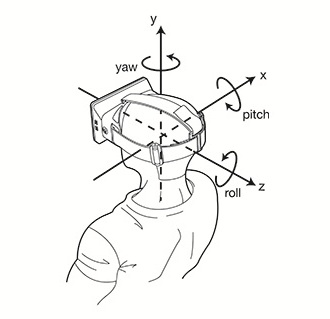
\includegraphics[scale=3]{OculusHead.jpg}
  \caption{\label{fig:ypr} The 3 angles characterizing the orientation of the head\protect\footnotemark}
\end{figure}
\footnotetext{Illustration from the OculusVR blog}

The Euler Integration is not an exact method and the gyroscope measurements are not 100\% accurate. Thus the true orientation is drifting away from the calculated orientation. Other sensors are needed to correct the orientation. The accelerometer is used for correcting the \textit{tilt error} -- where the up direction is -- while the magnetometer is used to correct the \textit{yaw error}.

\subsubsection{Correction of the tilt error}
The up direction is defined by the gravity and the acceleration vector, which is roughly $9.81m/s^2$. Using a three-axis accelerometer, we can measure this vector but also every other additional accelerations due to the movement of the headset. Since the drift is slow, two conditions have to be met before correcting the drift:
\begin{enumerate}
\item The length of the measured acceleration vector is around $9.81m/s^2$
\item The gyroscope reports that the rotation is very slow
\end{enumerate}
There are some flaws in this method. It is possible to cancel the gravity acceleration by moving down while creating a lateral acceleration of $9.81m/s^2$. However this method is simple enough and works in the vast majority of cases.

Once the acceleration vector $a$ is found, the angle $\phi$ between $a$ and the $z$-axis is computed. The rotation axis is called the tilt axis and correspond to $(-a_z, 0, a_x)$. Rotating along this axis of angle $\phi$ re-aligns the up direction correctly -- see Figure~\ref{fig:tilt}.

\begin{figure}[h]
  \centering
  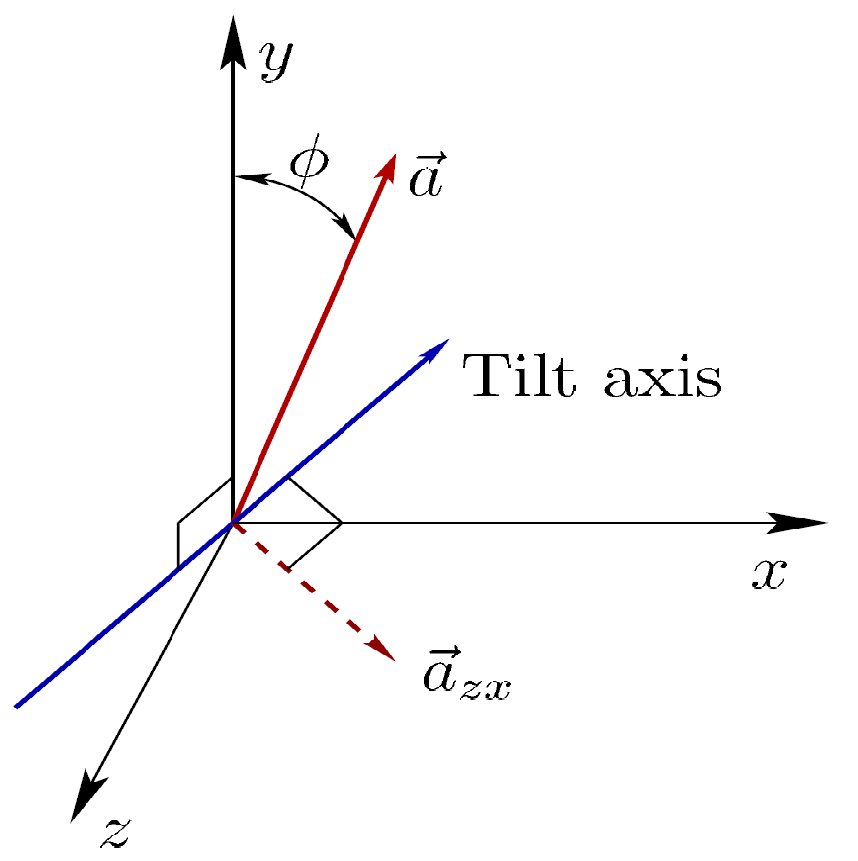
\includegraphics[scale=0.2]{tilt.png}
  \caption{\label{fig:tilt} Visulalisation of the tilt axis\protect\footnotemark}
\end{figure}
\footnotetext{Illustration from the OculusVR blog}

\subsubsection{Correction of the yaw error}
The yaw error is corrected by using the magnetic field of the Earth. The magnetic field of the Eart can be represented by a 3D vector field -- with magnitude and direction. Since the user of the Rift stays in the same area, the magnetic field is assumed to be constant. The magnetometer can not directly measure the absolute magnetic field $m = (m_x, m_y, m_z)$ because it measures the field relative to its own orientation. The three-axis magnetometer measures $m$ projected on each of its axes. Figure~\ref{fig:field} illustrates the issue in 2D.

\begin{figure}[h]
  \centering
  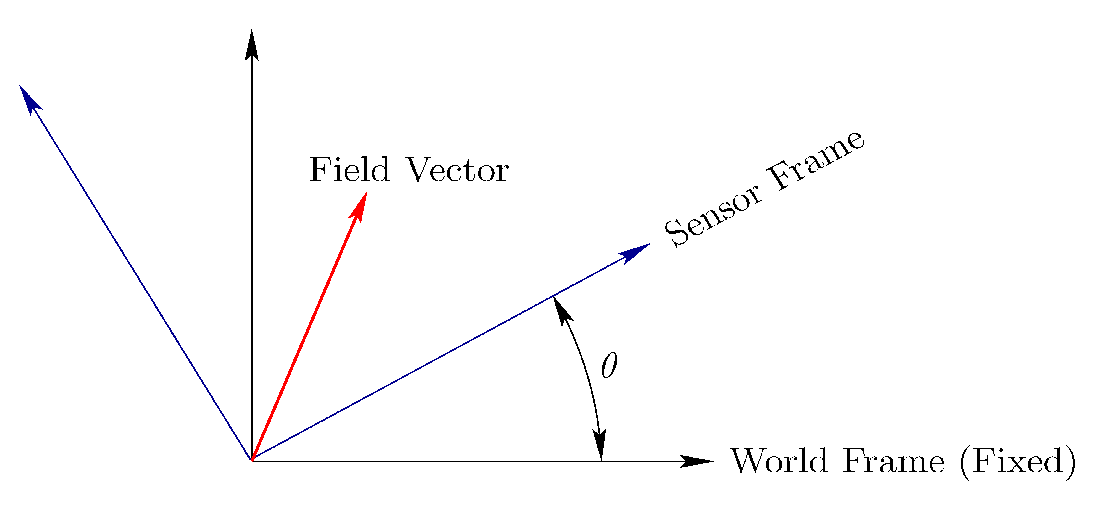
\includegraphics[scale=0.2]{RotMag.png}
  \caption{\label{fig:field} Measurement of the magnetic field\protect\footnotemark}
\end{figure}
\footnotetext{Illustration from the OculusVR blog}

If the sensor is rotated anticlockwise by angle $\theta$, then the measured field is rotated by $-\theta$. So a magnetometer readind from inside the rift gives a clue about its orientation based on the sensed magnetic field vector.

However, the Earth magnetic field is not the only one present in the everyday life. All electronic devices create a magnetic field. According to the Public Health England, the exposure level due to electrical appliances is close to 0.002 Gauss, whereas the Earth magnetic field is around 0.5 Gauss in the UK \cite{HPA}. So the magnetic fields from electronic devices can be neglected, except for the Rift itself. The Rift generate a constant magnetic field vector at the sensor, so a fixed offset is applied for each magnetometer sensor axis. By turning the Rift around through all orientations, the observed values should then lie on a sphere -- after noise filtering.

The readings of the magnetometers are then used for calibrating the Rift. Once it is calibrated, the drift is detected by using reference points. To save a reference point, the Oculus stores the magnetometer reading and the estimate of the Rift orientation. To detect a yaw drift error, the algorithm uses 4 steps:
\begin{enumerate}
\item Take the reference and transform the magnetometer into a world frame vector $m_w=(m_x,m_y,m_z)$ using the orientation -- quaternion -- at which it was stored.
\item Take the current magnetometer reading and transform it into a world frame vector $r_w=(r_x,r_y,r_z)$ using the current Rift orientation.
\item $r_w$ and $m_w$ are projected on the horizontal plane -- it is the same assuming the tilt error has already been corrected.
\item $\theta = atan2(m_z,m_x)$ and $\phi = atan2(r_z,r_x)$ gives us the yaw drift error $e = \theta - \phi$ with $e \in [-\pi,\pi]$.
\end{enumerate}

Knowing the yaw error, the orientation of the Rift is ajusted accordingly.

\subsection{Head mounted display and Lens deformation}
\label{subsec:lensdef}
The screen of the Rift -- sometimes called Head Mounted Display or HMD -- displays one image for the left part on the left part of the screen and one image for the right eye on the right part of the screen. The hardware is optimised for an interpupillary distance of 65mm. Two different images mean that we need to render the scene from two different points of view.

The lenses in the Rift magnify the images, thus providing an almost real-life field of view. However, the lenses distort the images a lot. If we display the original 3D image on the screen, then the user observes a pincushion distortion effect \cite{OVRDoc} -- see Figure~\ref{fig:pindist}.

To avoid this distortion, we must post-processed the 3D rendered views. We apply an equal and opposite barrel distortion -- Figure~\ref{fig:bardist} -- in order to cancel the puncushion distortion.

\begin{figure}[h]
        \centering
        \begin{subfigure}[b]{0.3\textwidth}
                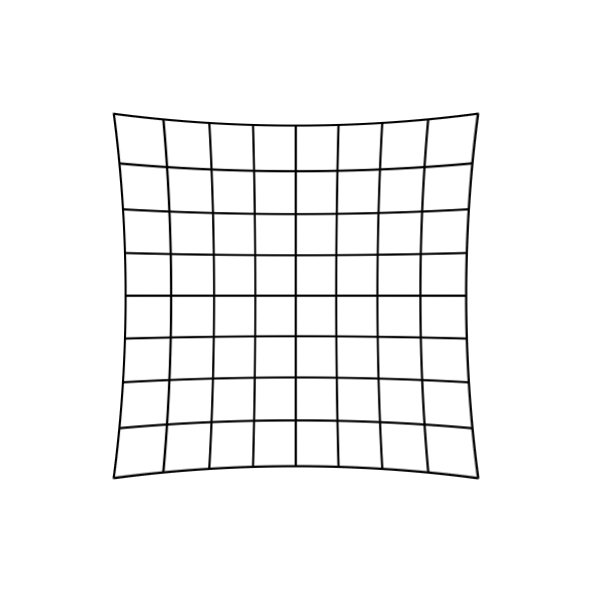
\includegraphics[scale=1]{PinDist.png}
                \caption{Pincushion distortion}
                \label{fig:pindist}
        \end{subfigure}
        \begin{subfigure}[b]{0.3\textwidth}
                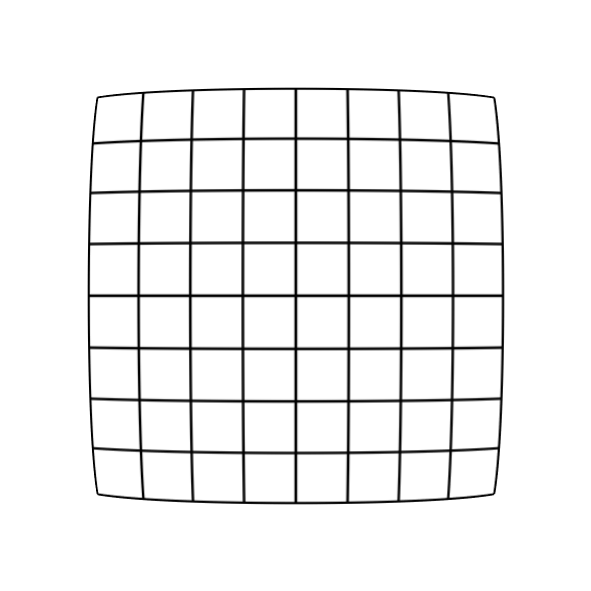
\includegraphics[scale=1]{BarDist.png}
                \caption{Barrel distortion}
                \label{fig:bardist}
        \end{subfigure}
        \caption{Distortion of the lenses}
\end{figure}

The lenses cause also chromatic aberrations on the edges of the field of view.

\newpage
\section{Implementation}
The implementation was made in C++ and in CUDA. It is based on kfusion, an implementation of KinectFusion developed by Gerhard Reitmayr.

\subsection{kfusion}
This project was the first time I was re-using an existing code. Before that, I always coded from scratch my projects or I was using libraries. With kfusion I had to understand how the whole code was functionning before starting to write code.

\subsubsection{Short description of the implementation}
The core of the software resides in \texttt{kfusion.h} and \texttt{kfusion.cu}. These two files describes the objects used for the volumetric integration and the tracking of the user. The object \texttt{KFusion} is the key of KFusion. It stores the volumetric description, the current and past vertex maps and normal maps.

\texttt{kinect.cpp} is the main file of kfusion. It contains the main loop for the volumetric integration, the pose estimation, the raycasting and displaying the rendered images. It also handles all the information about the Oculus Rift and its orientation. We use OpenGL only for displaying the image.

\texttt{helpers.cu} is the file that concentrates most of the rendering functions. It contains the rendering functions for the regular view and also for the Oculus distorted view.

\subsubsection{Choice of the parameters}
There are critical parameters to choose when using KinectFusion. Two of them are the size of the scene we want to map and the resolution of the corresponding volumetric representation. The size of the scene is in meters and corresponds to a cube. The resolution corresponds to the number of voxels along each axis.

Figures~\ref{fig:highres} and~\ref{fig:lowres} show the difference between a high-resolution parameter and a low-resolution parameter for the same volume size.

\begin{figure}[h]
        \centering
        \begin{subfigure}[b]{0.45\textwidth}
                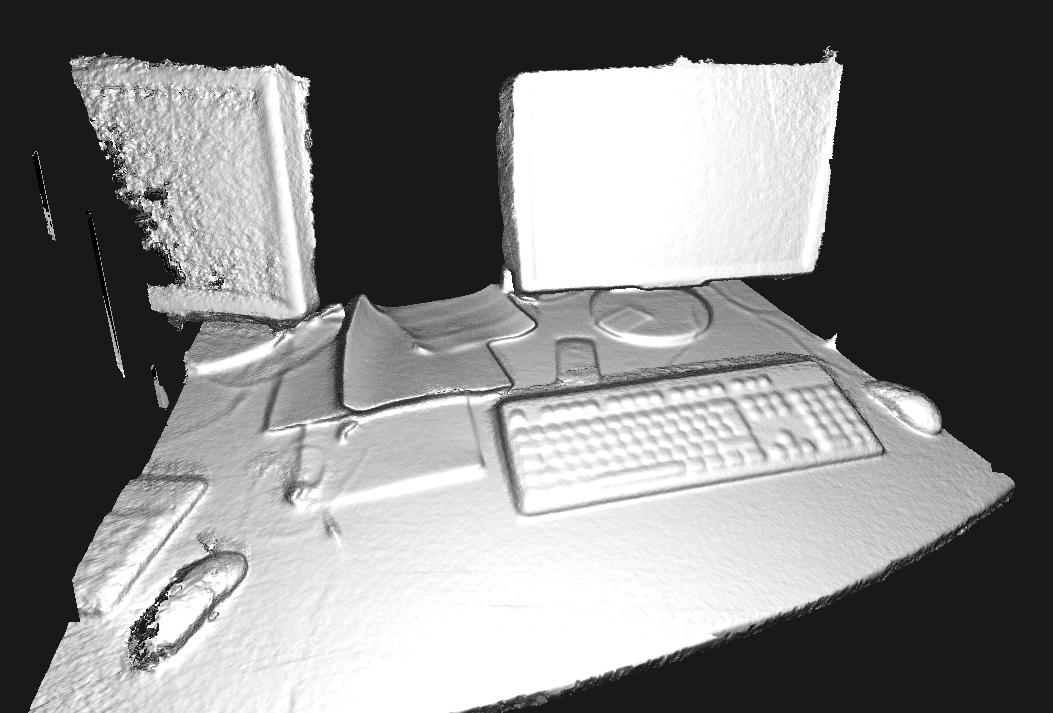
\includegraphics[width=1\textwidth]{HighRes.png}
                \caption{Volume size = 1m, Resolution = 700}
                \label{fig:highres}
        \end{subfigure}~
        \begin{subfigure}[b]{0.45\textwidth}
                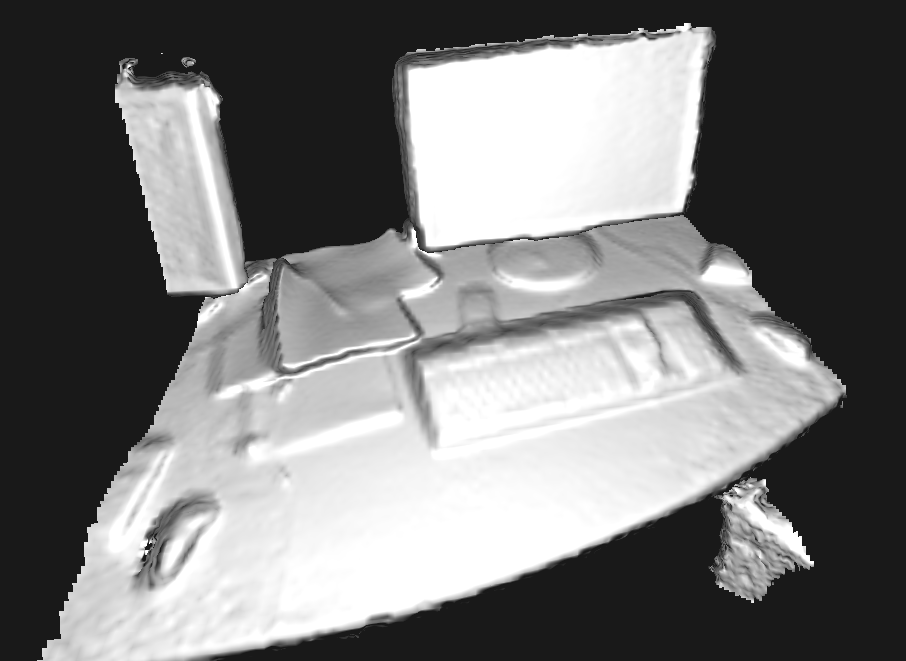
\includegraphics[width=1\textwidth]{LowRes.png}
                \caption{Volume size = 1m, Resolution = 128}
                \label{fig:lowres}
        \end{subfigure}
        \caption{Resolution parameter}
        
\end{figure}

Figures~\ref{fig:largevol} and~\ref{fig:smallvol} show the difference between a large volume parameter and a small volume parameter for the same volume size.

\begin{figure}[h]
        \centering
        \begin{subfigure}[t]{0.45\textwidth}
                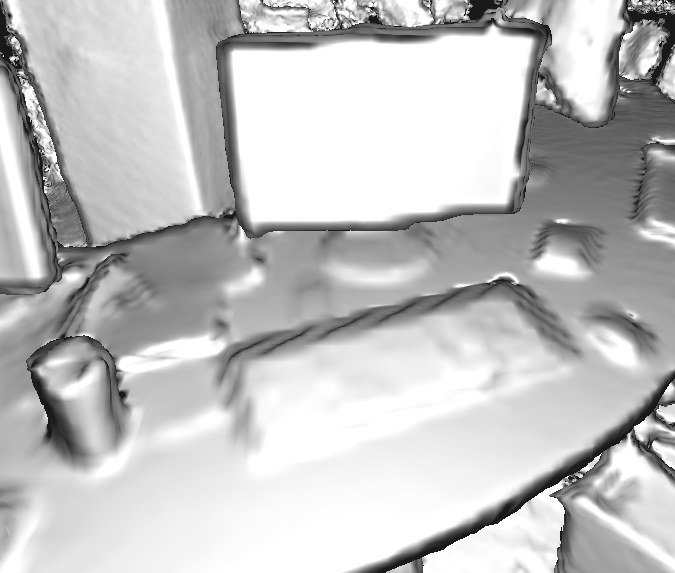
\includegraphics[width=1\textwidth]{VolLarge.png}
                \caption{Volume size = 10m, Resolution = 640}
                \label{fig:largevol}
        \end{subfigure}~
        \begin{subfigure}[t]{0.45\textwidth}
                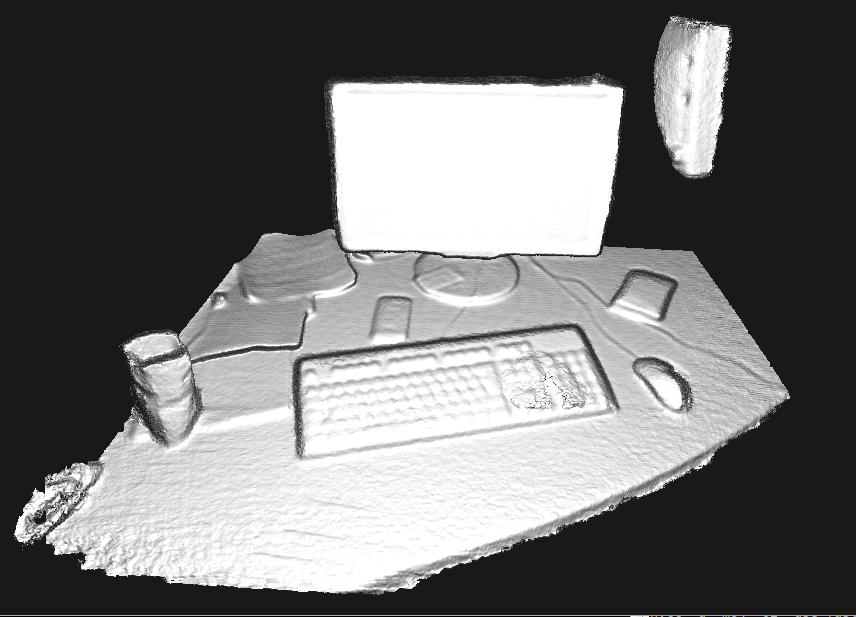
\includegraphics[width=1\textwidth]{VolSmall.png}
                \caption{Volume size = 1m, Resolution = 640}
                \label{fig:smallvol}
        \end{subfigure}
        \caption{Volume size parameter}
        
\end{figure}

Clearly, a high resolution gives a better looking result. However the higher the resolution, the more memory and computing power we ask from the GPU.

For our project, we need to combine a good resolution so that the user thinks the scene surrounding him is real. But we also need a large volume size so the user can move around in the scene. After multiple tests, we found that the best compromise was to choose a resolution of 700 with a volume size of 5m. Figure~\ref{fig:totalvol} shows the aproximate maximum area that can be mapped using these parameters.

\begin{figure}[h]
  \centering
  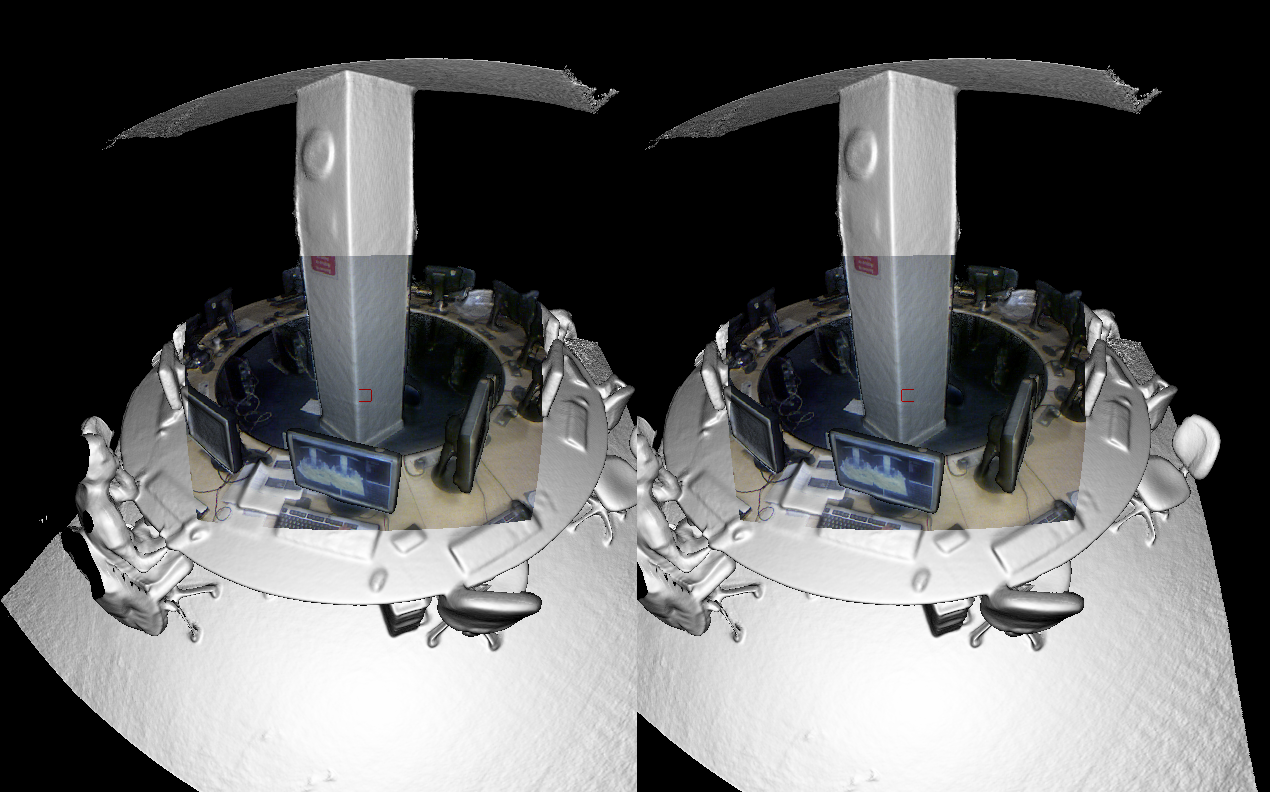
\includegraphics[scale=0.3]{TotalVol.png}
  \caption{\label{fig:totalvol} Approximate volume that can be mapped with parameters Volume size = 5m and Resolution = 700}
\end{figure}

\subsection{Lens deformation}
\label{subsec:deformation}
As said in subsection~\ref{subsec:lensdef}, we need to apply a barrel distortion to the image if we want to display it correctly in the Rift. Two methods are possible. The first one consists to render a normal 3D image and then distort it. The second method is to raycast directly with the lens model and not with the camera model.

\subsubsection{Rendering and distorting}
For the visualization inside the Rift, we need two renderings at two different points of view. We create two \textit{virtual cameras} either side of the Kinect camera. The two cameras are created from $K^{-1}$ by adding or subtracting an offset along the x-axis. Once we have the two modified matrices, we render the two scenes with the raycasting algorithm.

We know need to distort the two images. The Oculus SDK doesn't provide a tool for an already rendered image, but a model of the distorsion correction is given in \cite{OVRSDK}.

We tried to implement the distorsion for already rendered images. We encountered difficulties with it: we couldn't obtain focus for the whole image. By modifying some parameters, we could achieve focus in the foreground but not in the background and vice-versa.

Moreover, this method is not optimal. We have to render the two images and then warp them. These two steps could be combine into one using directly the Lens model for the ray casting.

\subsubsection{Lens raycasting}
The second method consist to raycast directly the distorted scene. The idea is to raycast using the lens model and not the camera model. This method avoid sampling problem when distorting the already rendered image. Given a pixel to render, we need to compute the corresponding direction for the raycasting.

The distortion model of the Lens transforms polar coordinates of an image $(r,\theta)$ as follows:
$$(r,\theta)\rightarrow (f(r)r, \theta)$$
with $f(r)$ being a \textit{scaling function} defined by
$$f(r)=k_0+k_1r^2+k_2r^4+k_3r^6$$
The direction $\theta$ is unchanged and the distance $r$ is expanded or contracted. In the case of the barrel distorsion, $k_0$, $k_1$, $k_2$ and $k_3$ are all positive. By choosing correctly these coefficients, the pincushion distorsion can be cancelled. $r = 0$ defines the principal point of the eye, meaning it is the direction where the pincushion distorion does not distort the image.

Code~\ref{lst:lensray} shows the transformation from a pixel coordinate $uv$ to a ray.
\clearpage

\begin{lstlisting}[language=C++, caption={C++ code for the Lens distortion}, label={lst:lensray}]
float f = 204.4f; // focal length
float2 iResolution = make_float2(1280, 800); // Size of the final image:
                                             // the Oculus Rift DK1 has
                                             // a resolution of 1280*800
float DistortScale = 1.71461;
float pp_adjust = 48.62;
float3 K = make_float3(1.00f, 0.22f, 0.24f); // Camera polynomial model
                                             // of the Lens

const uint2 pos = thr2pos2();
float2 uv = make_float2(pos.x, pos.y); // pixel coordinate
    
// Which eye?
float i = uv.x <= iResolution.x/2.0 ? 0.0 : 1.0;

// Compute Principle point
float sx = i*2.0 - 1.0;
float2 pp = make_float2(sx*(iResolution.x/4.0 - pp_adjust) + iResolution.x/2.0,
                        iResolution.y/2.0);

// Distort uv for Oculus (using resolution independant coords)
// assuming we have the right ratio between width and height
float2 theta = make_float2(4.0*(uv.x-pp.x)/iResolution.x,
                           4.0*(uv.y-pp.y)/iResolution.x);
float rSq= theta.x * theta.x + theta.y * theta.y;
uv.x = pp.x + iResolution.x*theta.x*(K.x+rSq*(K.y+rSq*K.z))/(4.0*DistortScale);
uv.y = pp.y + iResolution.x*theta.y*(K.x+rSq*(K.y+rSq*K.z))/(4.0*DistortScale);

float2 uvMinusPp = make_float2(uv.x - pp.x, uv.y - pp.y);
uvMinusPp.x /= f;
uvMinusPp.y /= f;

float3 ray = make_float3(uvMinusPp.x, uvMinusPp.y, 1.0f);
float rayNorm = sqrt(ray.x*ray.x + ray.y*ray.y + ray.z*ray.z);
ray.x /= rayNorm;
ray.y /= rayNorm;
ray.z /= rayNorm;
// ray is the direction for the raycasting
\end{lstlisting}

We compute the principle point on Line 18. The principle point is not the same for the left eye or the right eye since the lenses are not exactly centered. Then from Line 23 to Line 27 we apply the distortion directly using resolution independant coordinates -- that's why we divide by \texttt{iResolution.x/4}. The parameters of the scaling function are in \texttt{K} with $k_0 = 1$, $k_1 = 0.22$, $k_2 = 0.24$ and $k_3 = 0$.

Once the distortion has been computed, we compute the corresponding ray. With the focal length, the 2D coordinates uvMinusPp are taken back into the focal plan -- $z = 1$ -- giving us the direction for the raycasting. A comparison between the normal and distorted rendering is shown in Figure~\ref{fig:distortcomp}.

\begin{figure}[h]
        \centering
        \begin{subfigure}[t]{0.6\textwidth}
                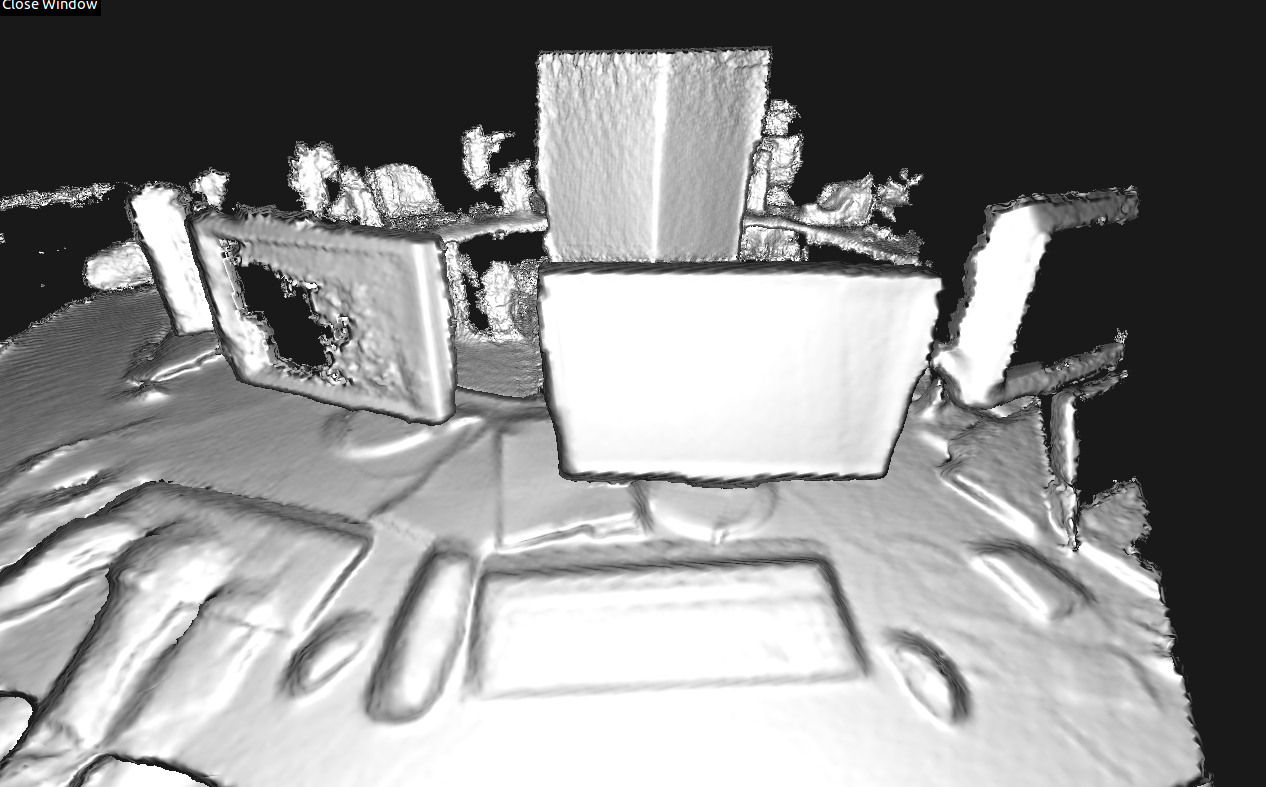
\includegraphics[width=1\textwidth]{BefDistort.png}
                \caption{}
        \end{subfigure}~\\
        \begin{subfigure}[t]{0.6\textwidth}
                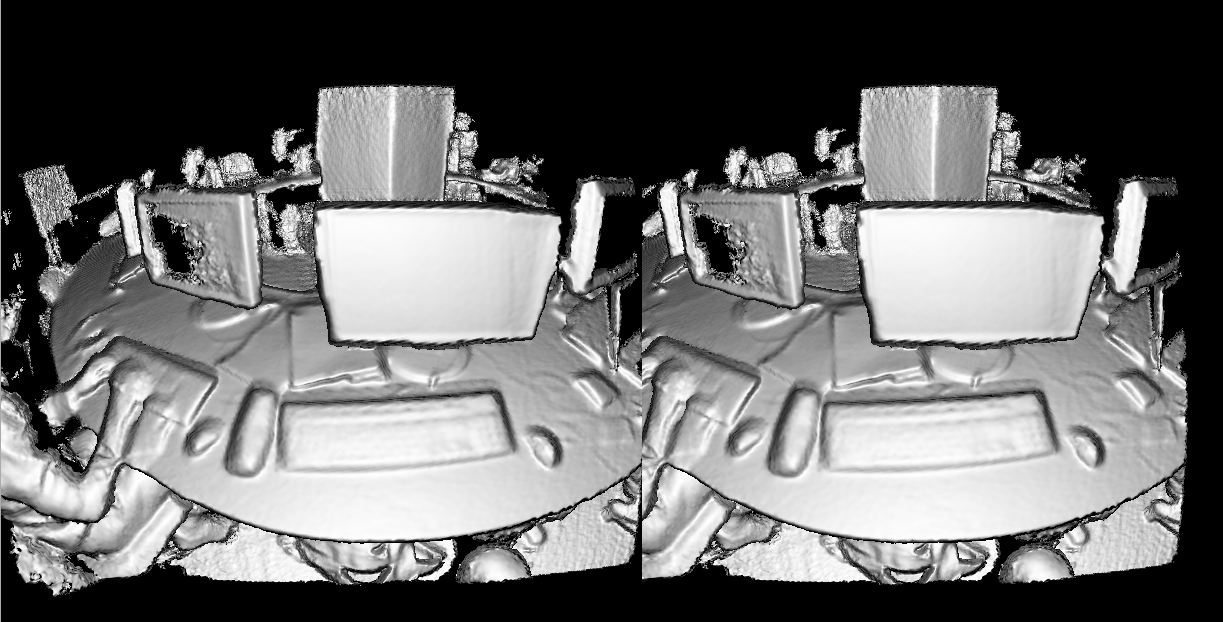
\includegraphics[width=1\textwidth]{AftDistort.png}
                \caption{}
        \end{subfigure}
        \caption{\label{fig:distortcomp}Before (a) and after (b) the Lens distortion}
        
\end{figure}

\subsection{Color rendering}
In the original KinectFusion implementation, color isn't displayed directly on screen. It is recorded, averaged and then displayed for an offline view of the recorded model. In our implementation, we want to use color since we want the user to be fully immersed in the surrounding scene: a gray-scale world is not realistic. We use the Kinect camera and project on the scene the live color information. This techniques provides a direct feedback of the scene, before the volumetric integration is even done. This way, the scene seems more natural to the user.

\subsubsection{Live color projection}
\label{subsubsec:colorprojection}
Once we raycasted a pixel, we want to find the corresponding pixel on the Kinect RGB image. We convert the 3D point back to non-global coordinates and then back to camera coordinates as follow:
$$u = KT_{i}^{-1}[x, y, z, 1]$$
$$p = [u.x/u.z, u.y/u.z]$$

$p$ is the corresponding pixel on the RGB image. If $p$ is out of bound, that means the raycasted pixel is not in the camera image. Therefore we render in gray scale. Else we have the color from the image and we can render the view in color. Figures~\ref{fig:nanb} and~\ref{fig:colorex} show the differences of a frame without colors and one with colors.

\begin{figure}[!h]
  \centering
  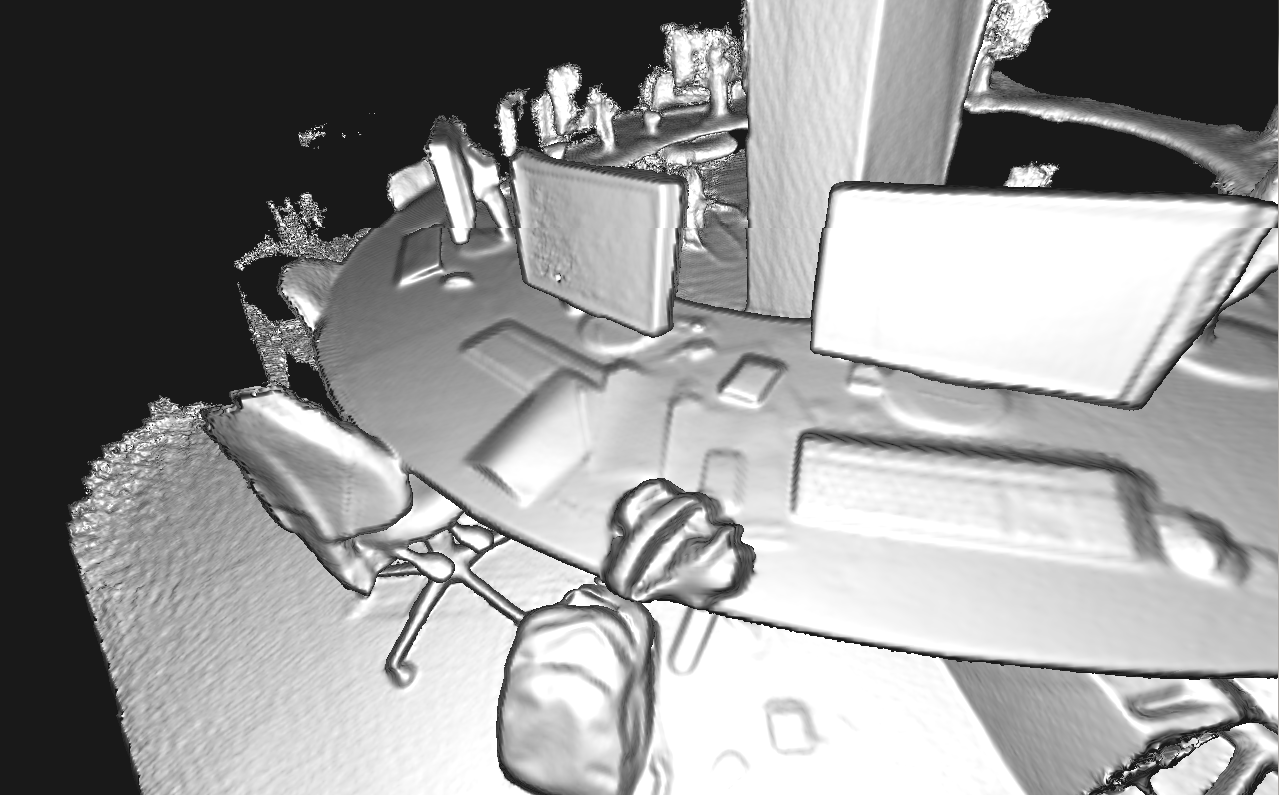
\includegraphics[scale=0.3]{NBExample.png}
  \caption{\label{fig:nanb} Scene without live colors}
\end{figure}

\begin{figure}[!h]
  \centering
  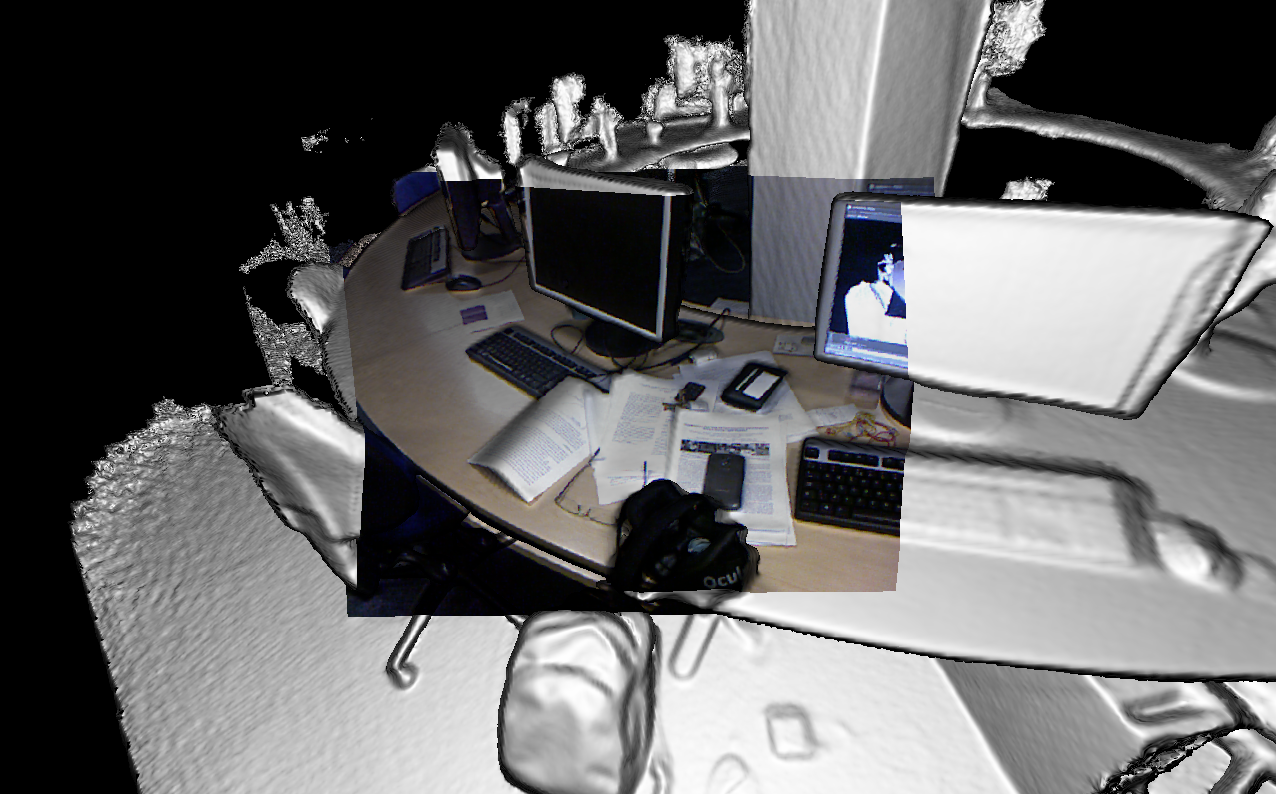
\includegraphics[scale=0.3]{ColorExample.png}
  \caption{\label{fig:colorex} Scene with live colors}
\end{figure}

Figure~\ref{fig:colorex} still shows a lot of grey scale areas. However we have to keep in mind that this image is then distorted with the barrel distortion -- see subsection~\ref{subsec:deformation}. With the barrel distortion and the human field of view, we can consider that almost 60\% of the field of view is seen in color. Figure~\ref{fig:oculuscolor} shows the Oculus distorted rendering with colors.

\begin{figure}[!h]
  \centering
  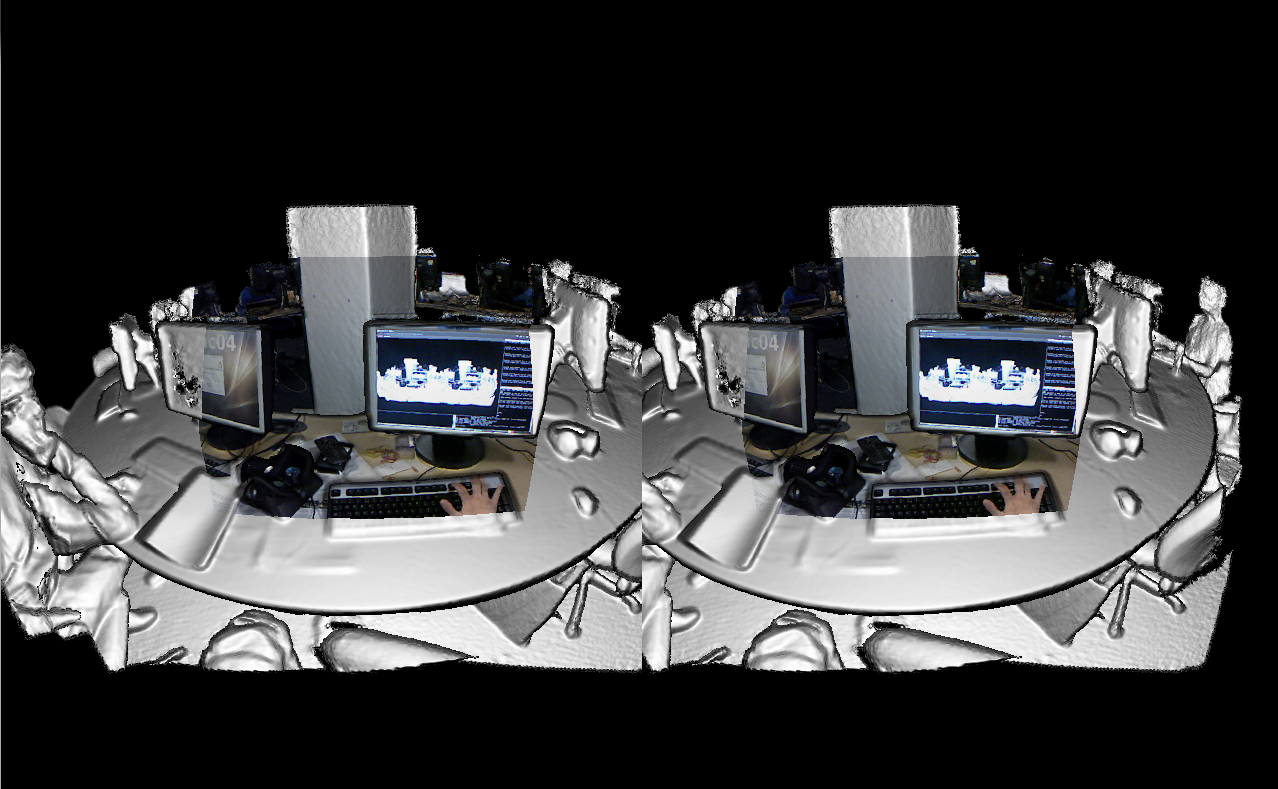
\includegraphics[scale=0.3]{ColorRift.png}
  \caption{\label{fig:oculuscolor} Scene displayed on the Oculus Rift with colors}
\end{figure}

\subsubsection{Issues using live color projection}
There are some issues when using live color projection. Because of the lag between the camera image and the rendering, the texture is sometimes misaligned with the model -- see Figure~\ref{fig:texture}.

\begin{figure}[!h]
  \centering
  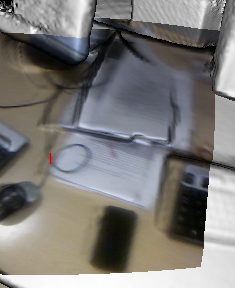
\includegraphics[scale=0.5]{TextureIssue.png}
  \caption{\label{fig:texture} The texture is not aligned with the model}
\end{figure}

The misalignement is better seen with high resolution for the volumetric representation. Because a high resolution is asking for more computational power, this creates a lag between the rendered image and the projected image. However we do not think that a high resolution volumetric representation is the only cause for this texture isssue. A combination of two effects is likely to explain a part of this phenomenon:
\begin{enumerate}
\item The RGB camera and the depth camera are not synchronised. The Kinect creates two images: a depth image -- called the depthmap, and a RGB image. But the two images are not computed at the exact time. When our program fetches the depth image and the RGB image, these two images are not from the exact same time, thus causing a shift between the model and the image.
\item The RGB camera is subject to the rolling shutter effect. The rolling shutter is a technique used by some cameras to take a picture. Instead of reading and writing the whole pixel array at once, the rolling shutter scans quickly horizontally or vertically the pixel array. The use of a rolling shutter creates distortion effects such as wobble and skew. These effects can affect the live projection and thus creates a misalignement with the model.
\end{enumerate}

Live color projection presents another small issue: the RGB camera of the Kinect automatically adjusts to the ambient light intensity. Because they are reflections on the desks in the lab, sometimes the user can be blinded by the reflection because the camera didn't already adjust to the new light intensity.

\subsection{Oculus Rift Calibration}

Our prototype is rudimentary. The Kinect is attached to the Rift thanks to paper clips and rubber bands -- see Figure~\ref{fig:prototype}. This cause multiples issues:
\begin{enumerate}
\item The Kinect can move slightly compared to the Rift. So the Kinect view direction is not the same as the Rift view direction. This is a prime issue because the user head position and orientation will not match the Kinect position and orientation. If the user is looking straight ahead and he sees his feet, it is going to confuse the brain -- and it will be painful if the user wants to really look straight ahead by tilting his head back.
\item The position of the Kinect is not the same as the user point of view. Because of the size of the Rift and the size of the Kinect, the distance between the point of view of the user and the point of view of the Kinect is around 20cm.
\end{enumerate}

\begin{figure}[!h]
  \centering
  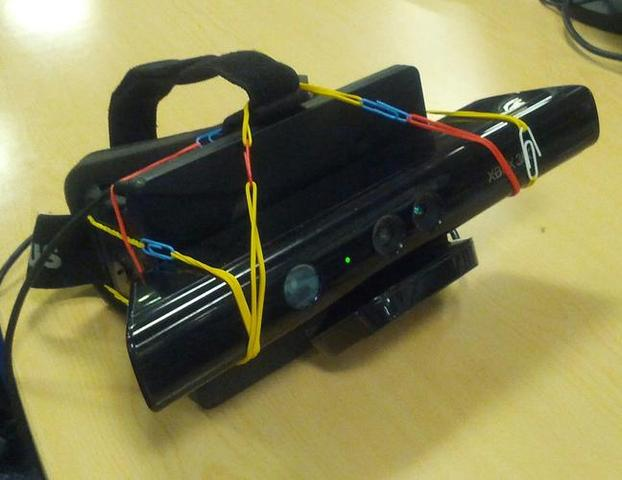
\includegraphics[scale=0.3]{Prototype.jpg}
  \caption{\label{fig:prototype} Our prototype}
\end{figure}

\subsubsection{Oculus orientation and Kinect orientation}
In order to correctly calibrate the Oculus orientation with the Kinect orientation, we have one requirement: the Kinect should be correctly aligned with the Rift when the program is launched. If the two devices are not aligned, there is no possibility to estimate the transformation between the Kinect space and the Oculus space.

Given that the two devices are correctly aligned, they have the same orientation. During the first loop of the algorithm, we compute the orientation of the Kinect -- more precisely the Rotation matrix $R_i$ -- and the orientation of the Oculus thanks to the gyroscope, magnetometer and accelerometer. The computation of the transformation between the two rotation matrices is done easily: the transformation is a rotation made of the rotation matrix $R_i$ multiply by the inverse of the rotation matrix of the Oculus Rift. The inverse of a rotation matrix is easy to compute since it is only the transpose of the rotation matrix. Code~\ref{lst:calibration} shows the code for the calibration.

\begin{lstlisting}[language=C++, caption={C++ code for finding the transformation between the Kinect and the Rift}, label={lst:calibration}]
Mat3 rotHMDtoKINECT;
Matrix4 hmdPose;
Matrix4 kinectPose;
Mat3 hmdRot = getRot(hmdPose);
Mat3 kinectRot = getRot(kinectPose);
Mat3 transHmdRot = transpose(hmdRot);
rotHMDtoKINECT = multiply(transHmdRot,kinectRot);
\end{lstlisting}

The rotation matrix of the Rift is compute from the Euler angles. The Oculus SDK has a function capable of returning the yaw, pitch and roll angles -- respectively the angle along the $y$-axis, the $x$-axis and the $z$-axis. Code~\ref{lst:euler} shows the computation of the rotation matrix of the Oculus Rift.

\begin{lstlisting}[language=C++, caption={C++ code for computing the rotation matrix of the Rift}, label={lst:euler}]
void viewMatrixUpdate(Matrix4 & ovrPose, float yYaw, float zEyeRoll, float xEyePitch){
  ovrPose.data[0].x = cos(yYaw)*cos(zEyeRoll)
                    + sin(yYaw)*sin(xEyePitch)*sin(zEyeRoll);
  ovrPose.data[0].y = cos(zEyeRoll)*sin(yYaw)*sin(xEyePitch)
                    - cos(yYaw)*sin(zEyeRoll);
  ovrPose.data[0].z = cos(xEyePitch)*sin(yYaw);
        
  ovrPose.data[1].x = cos(xEyePitch)*sin(zEyeRoll);
  ovrPose.data[1].y = cos(xEyePitch)*cos(zEyeRoll);
  ovrPose.data[1].z = - sin(xEyePitch);
        
  ovrPose.data[2].x = cos(yYaw)*sin(xEyePitch)*sin(zEyeRoll)
                    - cos(zEyeRoll)*sin(yYaw);
  ovrPose.data[2].y = sin(yYaw)*sin(zEyeRoll)
                    + cos(yYaw)*cos(zEyeRoll)*sin(xEyePitch);
  ovrPose.data[2].z = cos(yYaw)*cos(xEyePitch);
}
\end{lstlisting}

Once we have the rotation $R_{RtoK}$ between the Kinect and the Rift, we can use the Rift orientation for the rendering of the scene. The \textit{true} orientation of the Rift is easily calculated as $R_{RtoK}\times hmdRot$.

So the rigid transform matrix we use for the rendering is $[R_{RtoK}\times hmdRot,t_i]$. This matrix solves the issue of Kinect movement compared to the Rift position.

\subsubsection{Point of view correction}

Because of the size of our prototype, the Kinect position is approximately 20cm in front of the eyes of the user. Since the Kinect position is closer to the scene than the head position, users have a hard time trying to grab objects without multiple tries.

We adjust the position with the code presented in Code~\ref{lst:position}.

\begin{lstlisting}[language=C++, caption={C++ code for adjusting the position of the user}, label={lst:position}]
float3 viewDirection = make_float3(0,0,-0.15f);
float3 vecToAdd = rotateVec(ovrPose, viewDirection);
ovrPose.data[0].w += vecToAdd.x;
ovrPose.data[1].w += vecToAdd.y;
ovrPose.data[2].w += vecToAdd.z;
\end{lstlisting}

Here we adjust the position of the head by backing the position of the head of 15cm. Line 1 creates the vector for backing the position. \texttt{ovrPose} is the rigid transformation matrix mentioned in the previous subsection. We transform the vector from Oculus space coordinates to global coordinates by multiplying the rotation matrix with the vector. Then we move the position of the rigid transformation matrix in Lines 3, 4 and 5.

Figures~\ref{fig:notcorrect} and~\ref{fig:correct} shows the difference before the correction and after the correction.

\begin{figure}[!h]
  \centering
  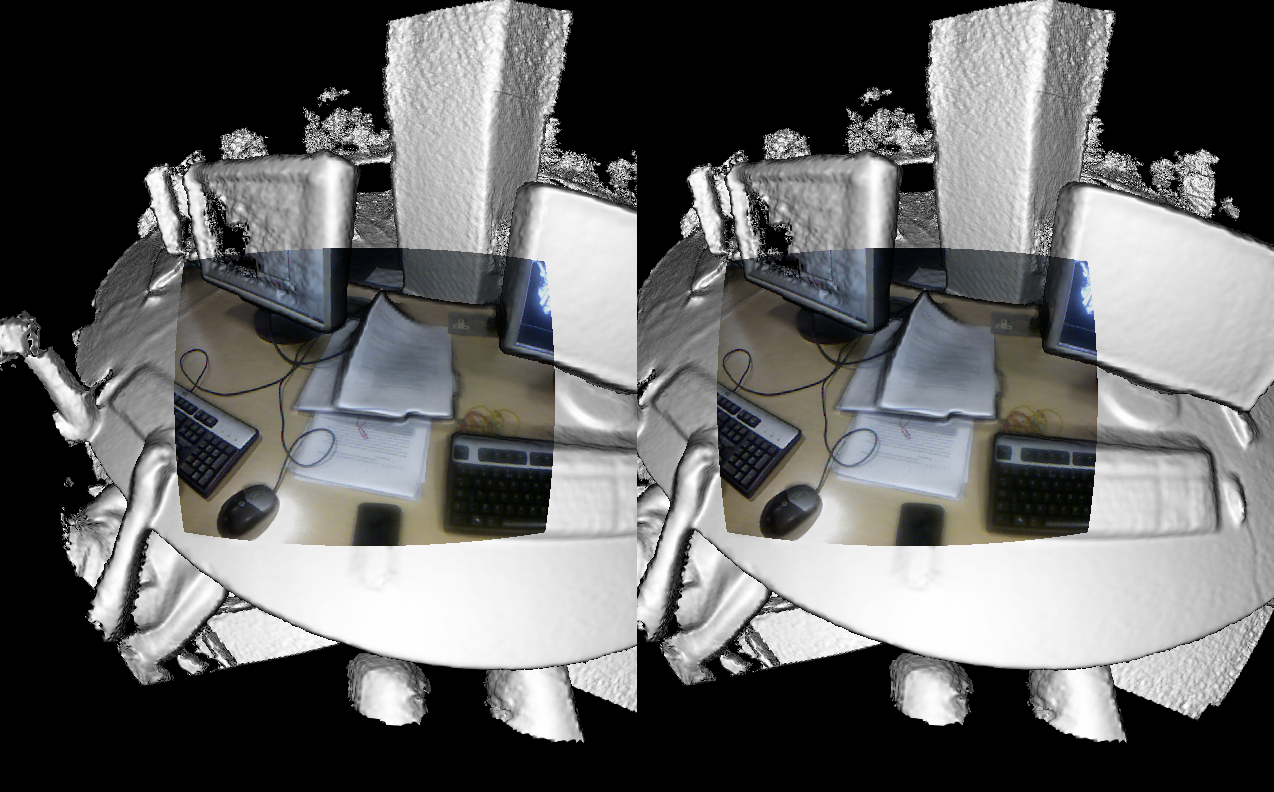
\includegraphics[scale=0.3]{NotCorrected.png}
  \caption{\label{fig:notcorrect} Rendered view before the correction}
\end{figure}

\begin{figure}[!h]
  \centering
  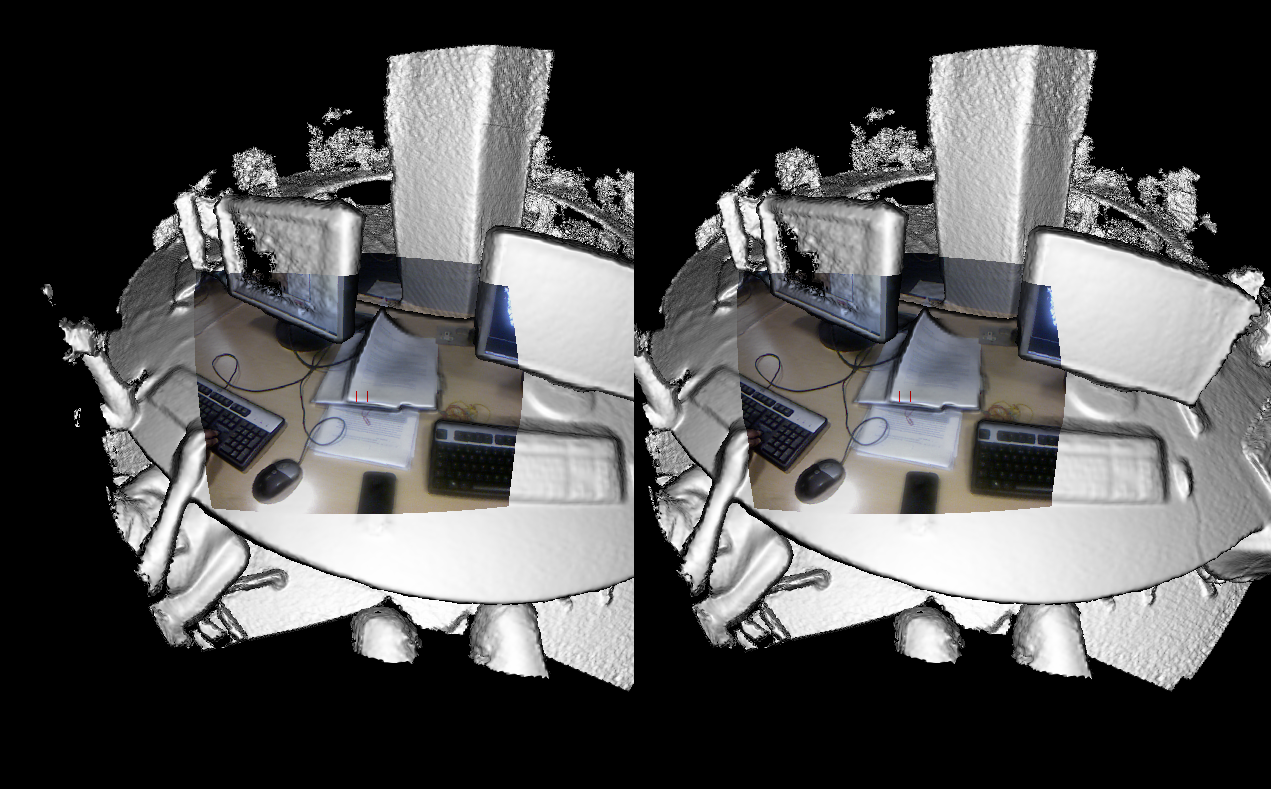
\includegraphics[scale=0.3]{Corrected.png}
  \caption{\label{fig:correct} Rendered view after the correction}
\end{figure}

\subsection{Magical Pen}
One of the goal of this project was to create an augmented reality application. We wanted to create an interactive application, not just a visual one. The original KinectFusion provided an augmented application where the user could draw on a surface with his/her hands. However, the visualization was difficult. The user was standing in front of the Kinect and didn't have a direct feedback of what he was drawing.

With the Oculus Rift, the user can see directly what he is drawing. It is then much more immersive.

\subsubsection{Tracking technology}
In the KinectFusion algorithm, the drawing application was tracking the hand of the user. Due to the proximity of the Kinect sensors in our prototype, hand tracking is difficult. We lack the depth information for providing a good tracking of the hand. In our implementation, we focused on color tracking of a pen.

To learn the color, we ask the user to place the color to be learned in the center of the view, symbolized on the screen by a red square. We convert the color information from the RGB space to the Hue Saturation Value space. This conversion allows a better tracking of a color. Even if the lighting condition changes, the Hue and Saturation of a color shouldn't change. This conversion makes the tracking more resistant and a pseudo-code is given in Algorithm~\ref{algo4}.

\begin{algorithm}
\caption{Conversion from RGB to HSV}\label{algo4}
\begin{algorithmic}[1]
\State float $red$, $gre$, $blu$
\State $max$ = max($red$,$gre$,$blu$)
\State $min$ = min($red$,$gre$,$blu$)
\If{$max = min$}
  \State $hue = 0$
\ElsIf{$max = red$}
  \State $hue = (60*(gre-blu)/(max-min) + 360)$
  \If{$hue > 360$}
    \State{$hue -= 360$}
  \EndIf
\ElsIf{$max = gre$}
  \State $hue = (60*(blu-red)/(max-min) + 120)$
\Else
  \State $hue = (60*(red-gre)/(max-min) + 240)$
\EndIf
\If{$max = 0$}
  \State $sat = 0$
\Else
  \State $sat = 1-min/max$
\EndIf
\State $val = max$
\end{algorithmic}
\end{algorithm}

HSV space uses 3 components : the hue, the saturation and the value. The hue is encoded according to its angle on the color wheel, therefore $hue \in [0;360]$. The saturation corresponds to the intensity of the color and $sat \in [0;1]$. Finally, the value corresponds to the brightness of the color and $val \in [0;1]$. If the lighting intensity is to change during the color tracking, only $val$ should vary. However, under a bright light or in the dark, the saturation and hue is difficult to compute due to the noise of the camera.

To determine which color to track, we take the mean color in a 20 by 20 pixels square. Since the hue is a circular value, extra care has been taken to compute the average.

The tracking keeps track of the latest known 2D position of the pen in the image. The tracking is done as follows:
\begin{enumerate}
\item In a square of 50 by 50 pixels -- represented by an array -- around the latest known 2D position, we look up every pixel. If the color of the pixel is close to the hue and saturation of the tracked color, we set its value to 1 in the array. Else we set it to 0.
\item We then compute a heatmap. For every pixel in the square previously introduced, we add all the values of the surrounding pixels in a specified radius.
\item Finally, we update the tracked position to the pixel position with the highest score on the heatmap.
\end{enumerate}

This algorithm works well and fast, given that the tracked color is not a color present in the background. In the lab, the tables are light brown, the walls are white, the floor is dark blue and the keyboards are black. By choosing purple as the color to track, we don't have interference with the background.

The threshold for the color comparison are the followings: $\left\| hue_{tracked} - hue_{pixel}\right\| < 0.2$ with the values in radians; $\left\| sat_{tracked} - sat_{pixel}\right\| < \dfrac{sat_{tracked}}{4}$.

\subsubsection{Computing the 3D position}
Once we have the 2D position, we need to compute the corresponding 3D position to know if the pen is in contact of a surface or not. We first compute the distance between the camera and the pen. We use the raw depth map from the Kinect. We compute the median distance for all the pixels within a certain radius of the tracked position. Here we use a 6 by 6 pixels square. This computed distance is once again filtered: we take the median of the last 10 computed distances. These two filters help prevent the misreadings of the Kinect sensor or the bad readings when the tracked position is on the edge of the pen.

Once we have the distance $d$ between the camera and the pen, we only need the direction vector from the camera to the pen. Considering the tracked position is note $u$, the direction vector is:
$$dir = R_iK^{-1}[u,1]$$
where $R_i$ is the current orientation pose of the Kinect and K the Kinect camera parameters. Once this vector $dir$ is normalized, we find the global 3D position of the pen:
$$pen^g = t_i + d*dir_{norm}$$
where $t_i$ is the current position of the Kinect.

\subsubsection{Writing on the surface}
Now that the successive positions of the pen are known, we have to colorize the parts of the scene where the pen wrote. We tried two different techniques for rendering the drawings. The first technique uses a vector, which stores all the positions of the pen. For every pixel to be rendered, we have a 3D position -- computed thanks to the raycasting. We compute the distance between the pixel position and the positions of the pen. If this distance is smaller than a threshold, the pixel is colorized in blue.

The main problem with this method is that it is extremely slow. With 5 stored positions in the position vector, the rendering is running at 10-15 frames per second. With 20 stored positions in the position vector, the rendering is running lower than 1 frame per second.

In order to limit the number of positions stored in the vector, we filter the incoming position: if the distance between the incoming position and the last position in the vector is smaller than a threshold, we don't add the incoming position to the vector. This simple filtering step prevents us to add a new position for every frame and thus limits greatly the number of stored positions. However, the filtering step is not sufficient for the rendering to run smoothly.

The second technique is based on a 3D grid. We divide the space with a grid of voxels. Each voxel stores a boolean. The grid is initialized to false for every voxel. When we compute the 3D position of the pen, we look at the corresponding voxel and set its value to true. Then when we render a pixel, we look at the corresponding voxel. If the value stored is true, we colorize the pixel.

Using a 3D grid is memory expensive. In our implementation, we use voxels with a size of 5mm forming a $1000*1000*1000$ voxels grid. Since a boolean has a size of 1 byte, the grid occupies 1GB of memory. On the other hand, the rendering is running smoothly, even after a long run time.

There are some drawbacks when using the 3D grid. The first drawback is the aspect of the drawing. Because we are using a voxel grid, the drawings look pixelated. Another issue is that the pen position isn't always correctly detected. The misdetection can leave a gap in the drawing. To solve this issue, we do not only set the value of the corresponding voxel to true but also the neighboring voxels.

\subsubsection{Results}
The Magical pen gives good results. Figures~\ref{fig:pen1} and~\ref{fig:pen2} show drawings rendered in the Rift.
\begin{figure}[!h]
  \centering
  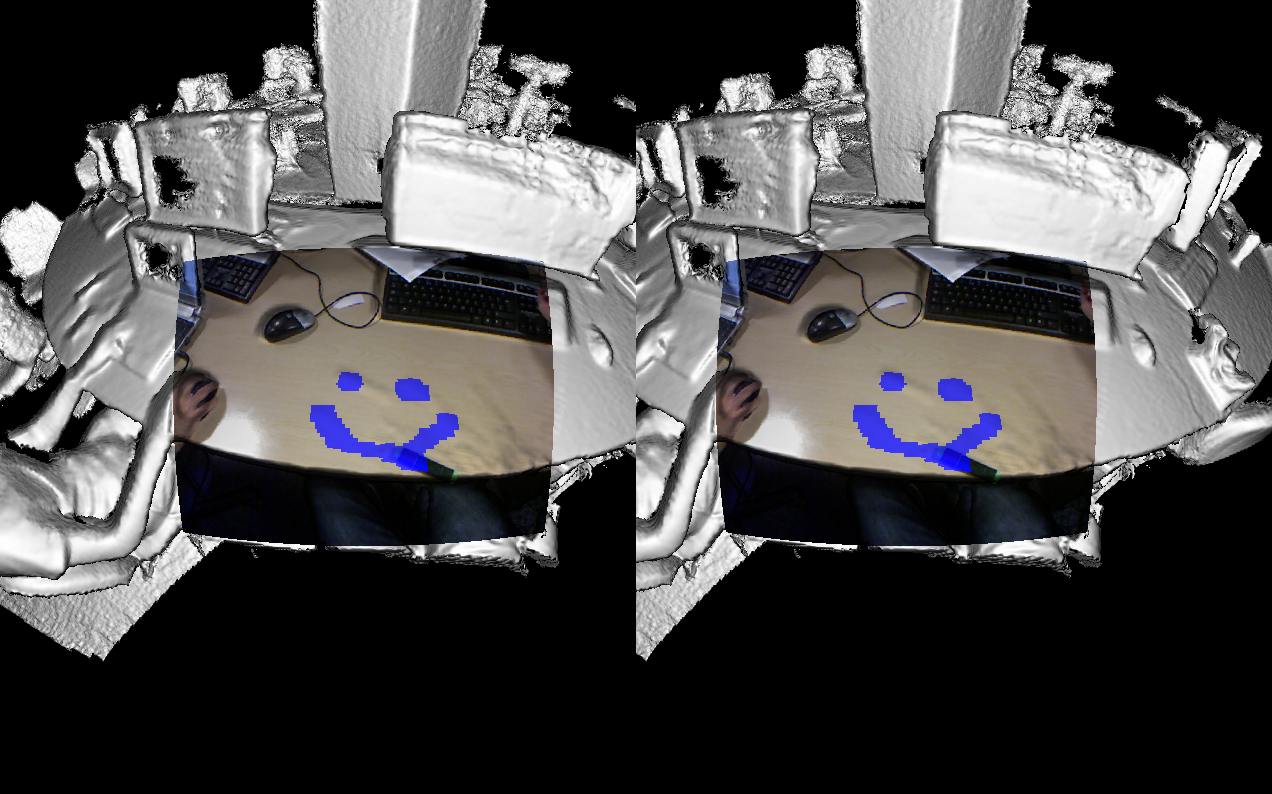
\includegraphics[scale=0.3]{pen1.png}
  \caption{\label{fig:pen1} Drawing in augmented reality}
\end{figure}

\begin{figure}[!h]
  \centering
  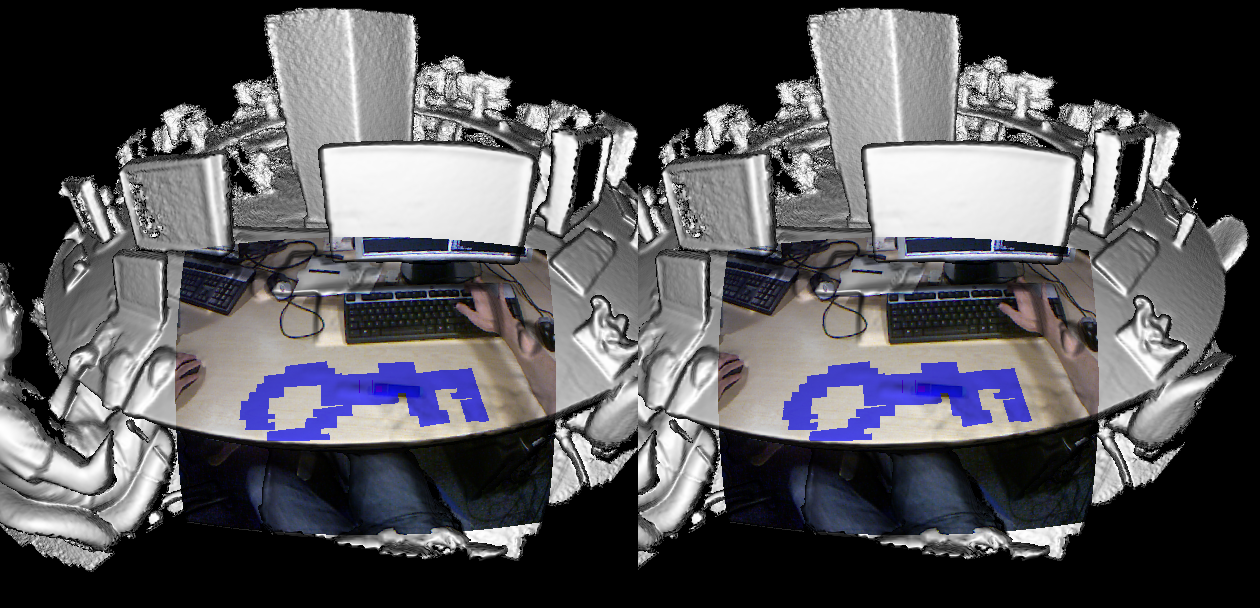
\includegraphics[scale=0.3]{pen2.png}
  \caption{\label{fig:pen2} Drawing in augmented reality}
\end{figure}

However, there are still some issues with the magical pen. Figure~\ref{fig:nowrite} shows a case where the pen is correctly tracked and the Kinect computes a valid depth whereas there is no writing on the surface.

\begin{figure}[!h]
  \centering
  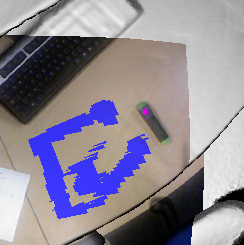
\includegraphics[scale=0.4]{NoWrite.png}
  \caption{\label{fig:nowrite} The pen is tracked but there is no writing on the surface}
\end{figure}

We noted that this issue mostly occurs when the pen is on the edges of the Kinect depthmap. When the pen resides at the center of the Kinect depthmap, the drawing is working fine. One explanation is that the depth returned by the Kinect doesn't match the actual distance between the Kinect and the pen. The distance returned by the Kinect appears to be shorter than the actual distance between the Kinect and the pen.

We verified our assumption by reproducing the issue and then placing a box in front of the pen position. Because the depth return by the Kinect was shorter, the pen wrote on the box even if it wasn't there. Indeed we note that the box has drawings on it, verifying the fact that the Kinect return a shorter depth when the pen is on the edge of the depthmap. Figure~\ref{fig:penissue} illustrates the proof.

\begin{figure}[h]
  \centering
  \begin{subfigure}[t]{0.5\textwidth}
    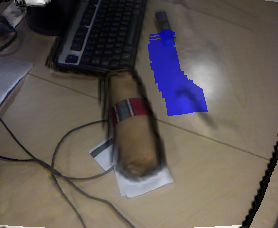
\includegraphics[width=1\textwidth]{PenIssue1.png}
    \caption{}
  \end{subfigure}~
  \begin{subfigure}[t]{0.5\textwidth}
    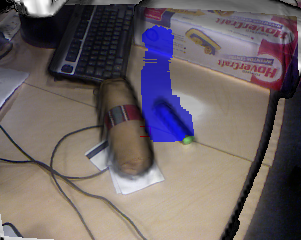
\includegraphics[width=1\textwidth]{PenIssue2.png}
    \caption{}
    \end{subfigure}
  \caption{\label{fig:penissue}In (a), the top of the pen is not colored in blue whereas it is currently being tracked. In (b) we placed a box in front of this pen position: drawing appears on the box, confirming the position recorded by the Kinect is shorter than the actual distance.}
  
\end{figure}

The tracking is quite robust since we are using the HSV space. The tracking can be lost if the pen is put under a bright light or a reflection -- we failed at computing the correct hue and saturation because we are too close to a white color.

\newpage
\section{Results}
\subsection{Hardware}
Our implementation was written in C++ and CUDA. The program was running on a computer with Ubuntu 13.04, an Intel Xeon QuadCore E5606 2.13GHz, 8GB of memory and a GPU NVidia GeForce GTX 780. We use the Kinect for Xbox 360 as depth sensor and the Oculus Rift development kit 1.
\subsection{3D rendering}
The KinectFusion implementation is running smoothly on the computer at more than 30fps. With the parameter volume size set to 5 meters and the resolution to 700, this is what a whole scene can look like -- Figure~\ref{fig:totalscene}.

\begin{figure}[!h]
  \centering
  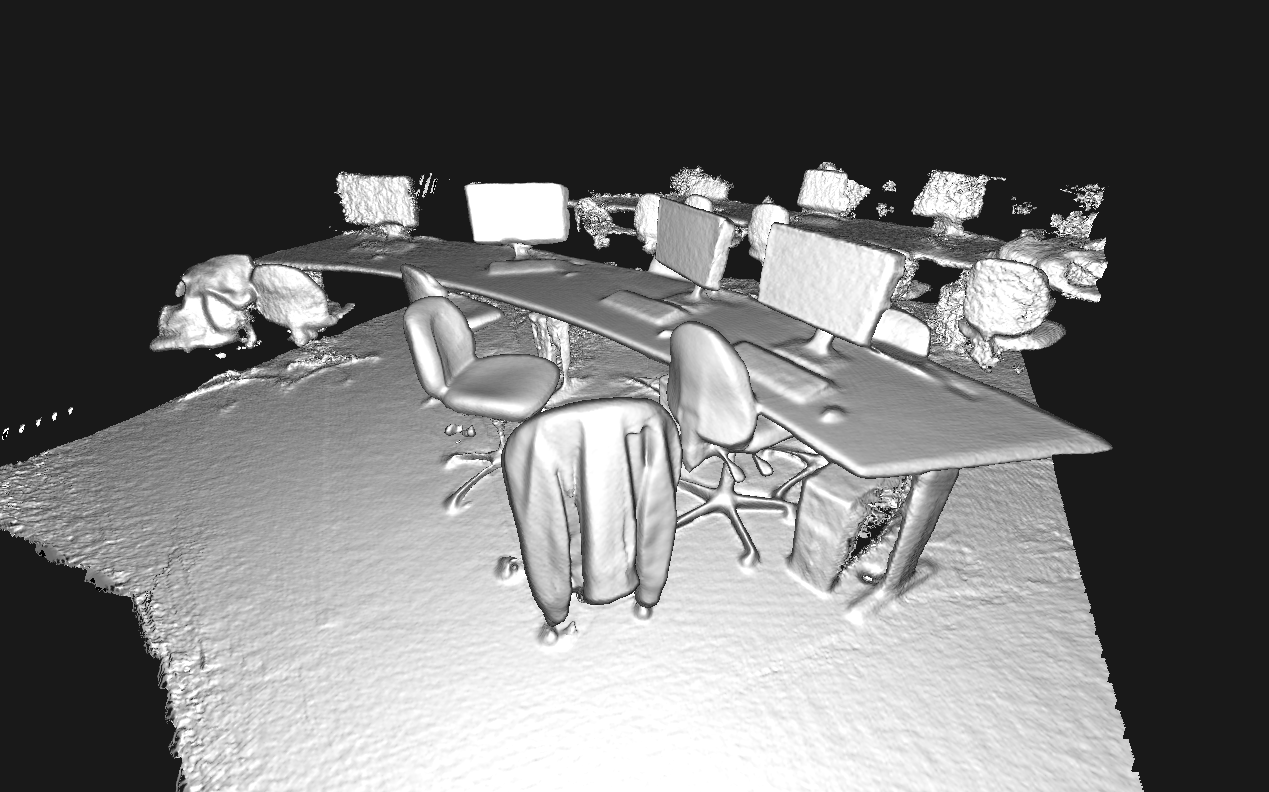
\includegraphics[scale=0.3]{WholeScene.png}
  \caption{\label{fig:totalscene} A scene with size = 5m and resolution = 700}
\end{figure}

The reconstruction is accurate, however we can spot minor glitches due to the raycasting -- see Figure~\ref{fig:glitch1} and Figure~\ref{fig:glitch2}.

\begin{figure}[!h]
  \centering
  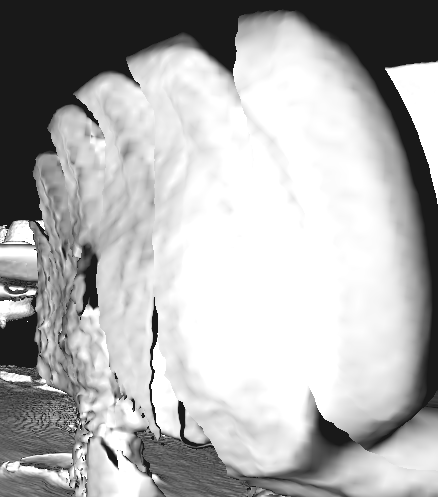
\includegraphics[scale=0.3]{glitch1.png}
  \caption{\label{fig:glitch1} Raycasting glitch}
\end{figure}

\begin{figure}[!h]
  \centering
  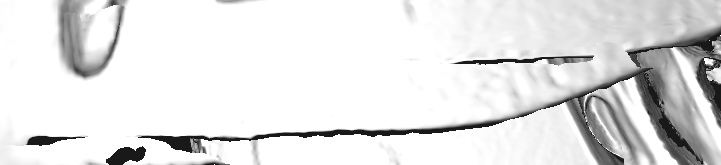
\includegraphics[scale=0.3]{glitch2.png}
  \caption{\label{fig:glitch2} Raycasting glitch}
\end{figure}

These glitches appear because the TSDFs are not exact when one angle of the scene has not been scanned. So before the TSDFs are updated, the raycaster is using the old ones, causing that kind of glitches. By properly scanning all the sides of an object, the glitches don't appear.

Another glitch can appear when someone is walking in the very background. Because the Kinect is not able to evaluate the actual distance with the scene once the person has leaved -- it is too far to reach for the IR pattern, the TSDF is not updated. So the recorded TSDFs is creating a glitch, shown in Figure~\ref{fig:glitch3}.

\begin{figure}[!h]
  \centering
  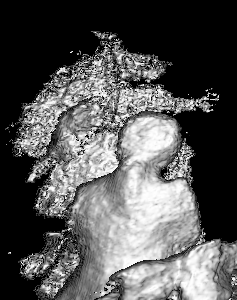
\includegraphics[scale=0.5]{glitch3.png}
  \caption{\label{fig:glitch3} TSDFs are not updated because the background is too far, creating this glitch.}
\end{figure}

Even with the low resolution RGB camera, the live color reprojection is giving good results. Figure~\ref{fig:color1} is the live color projection of a pillar from the lab. The clock is easily readable and so is the information panel beneath it. Figure~\ref{fig:color2} shows that the keys on the keyboard are almost readable.

\begin{figure}[!h]
  \centering
  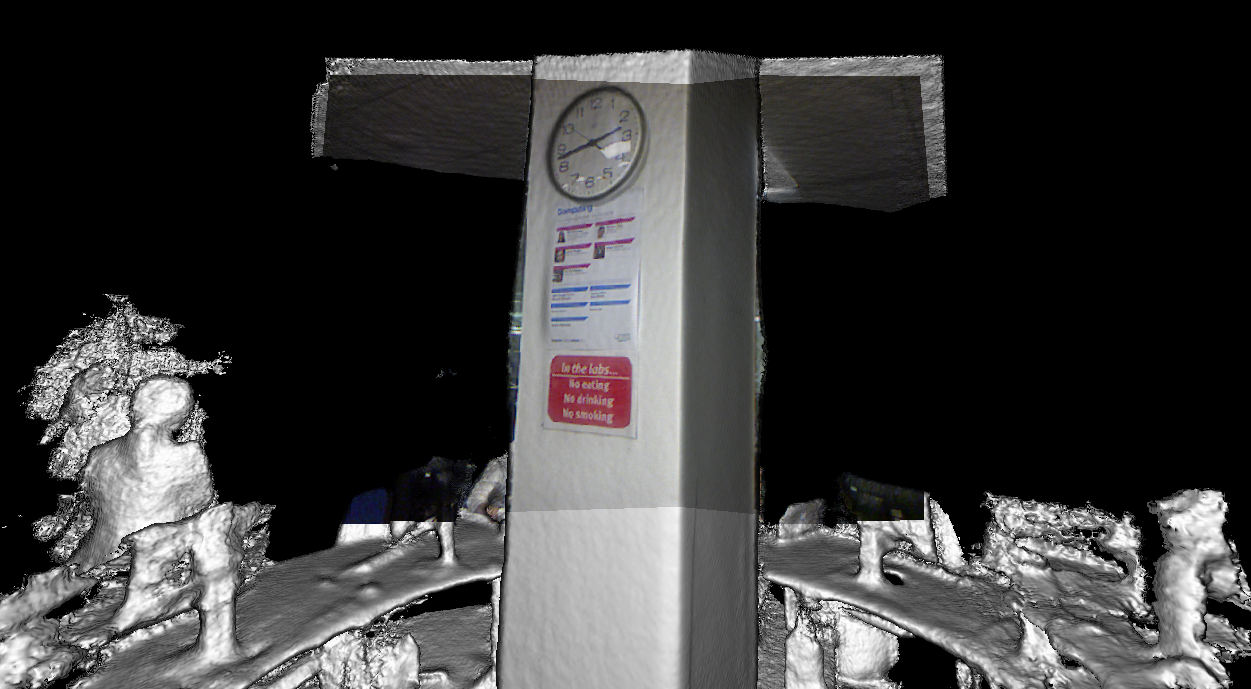
\includegraphics[scale=0.33]{Color1.png}
  \caption{\label{fig:color1} It is 2:43pm and we still can't eat or drink in the lab}
\end{figure}

\begin{figure}[!h]
  \centering
  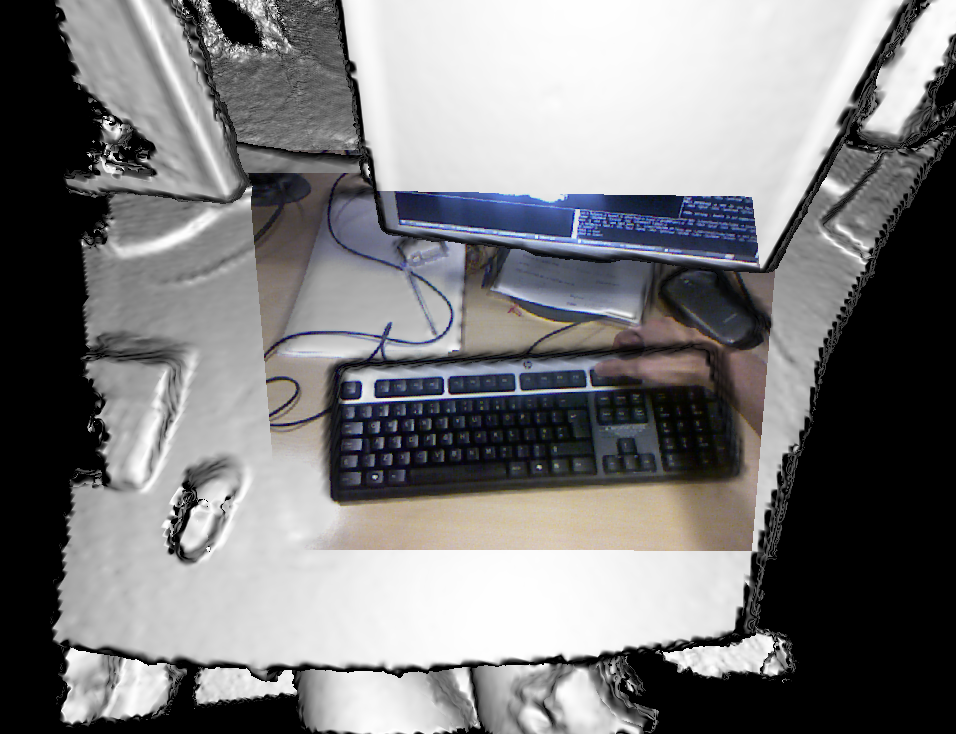
\includegraphics[scale=0.3]{Color2.png}
  \caption{\label{fig:color2} The keys on the keyboard are almost readable}
\end{figure}

Set apart the texture issue we already talked about, there is no noteworthy trouble with the live color projection.

\subsection{Magical pen}
The Magical pen is a great feature and it is has nearly no impact on the framerate of our program. We use a grid of $1000\times 1000\times 1000$ voxels, so a voxel has a side of 5mm. Figure~\ref{fig:hashtag} shows a writing on a table of the Computing Lab.

\begin{figure}[!h]
  \centering
  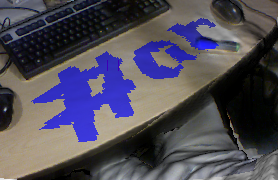
\includegraphics[scale=0.6]{hashtag.png}
  \caption{\label{fig:hashtag} Augmented reality drawing on a table}
\end{figure}

The drawing accomodates very well with changes in the orientation. Figure~\ref{fig:orientation} shows the same drawing under different orientations.

\begin{figure}[h]
  \centering
  \begin{subfigure}[t]{0.5\textwidth}
    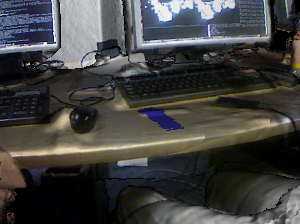
\includegraphics[width=1\textwidth]{Orientation1.png}
    \caption{}
  \end{subfigure}~
  \begin{subfigure}[t]{0.5\textwidth}
    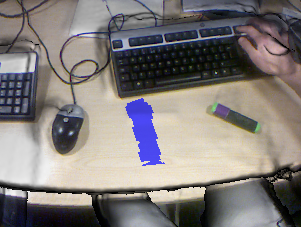
\includegraphics[width=1\textwidth]{Orientation2.png}
    \caption{}
    \end{subfigure}~\\
  \begin{subfigure}[t]{0.5\textwidth}
    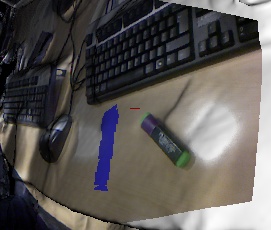
\includegraphics[width=1\textwidth]{Orientation3.png}
    \caption{}
    \end{subfigure}
  \caption{\label{fig:orientation} The same drawing is viewed at different orientations. As long as the Kinect tracking is effective, the drawing stays in place.}
  
\end{figure}

\newpage
\section{Future work}
Our prototype is working correctly, but it is still limited. In this part, we discuss the features that we would add if we had more time to develop them.
\subsection{Color rendering}
One of the major issue of our prototype is that not all the field of view of the user is in color. As we said in~\ref{subsubsec:colorprojection}, the color projection covers roughly 60\% of the user field of view. To reinforce the immersion, we need to take care of the last 40\%.

Multiple solutions can be considered. The first one would be to use another camera to capture the color in front of the user. A fish-eye camera could record the whole scene in front of the Rift. This would allow us to use live color projection for the entire view rendered for the user. This solution has numerous challenges. The first one is that we need a small fish-eye camera. The Kinect+Rift association is quite heavy as it is, so we have to keep the camera small. We also have to be able to find a correspondance between the rendered scene and the color frame taken by the camera. This implies that the camera has to be firmly attached to the Rift or the Kinect, so that its orientation is always known. The last task is to find the correspondance between the camera image and the rendered scene. Using a wide-angle webcam, we could be able to achieve a larger live color projection.

If we can't use another RGB camera, an alternative solution is to record the color in each voxel of the volumetric representation. When the Kinect first sees a voxel of the volumetric representation, we also record the average color of the voxel. Then if the voxel is out of the field of view of the RGB camera, we use this average color instead of rendering in shade of gray. This solution is simple to implement but can be memory expensive depending on the resolution of the volumetric representation. We need to store 3 values in each voxel, in other words we multiply by 2.5 the space required by the actual representation.

The main advantage of this last solution is that we are sure the whole scene is rendered in color. Using a good resolution, the result would be convincing. But it also comes with a major drawback: the camera takes the last known color as the color of the voxel. If an object comes in front of the camera, its color is assigned to the background since the volumetric integration takes some time to process. So a wrong color could be assigned to a voxel and creates oddities in the full colored redenred view. We can counter this effect by weighting the color just like we weight the depth for the volumetric integration. Using a weight would slow the color change so if the object doesn't stay in front of the surface too long, it won't have an effect on the registred color. For example, if a hand moves in front of the scene, the color wouldn't change right away.

\subsection{Hand-tracking}
Another useful capability would be a hand-tracking module. Right now it is almost impossible to track correctly the hands with the Kinect sensor: the hands are to close to the Kinect so we can't record the depth. Tracking the hands is interesting becomes it means the user can easily and naturally interact with the real world and the virtual world around him. It is a step forward for a better augmented reality experience.

Using the RGB camera, we can tracked the hands in 2D. \cite{Hand2D} proposes a method using Bayesian filtering and edge detection. This method can give us a pose estimation of the hand, but not the global 3D position of the hand. We could infer the approximate 3D position from the size of the hands or the length of the arms.

For tracking the hands in 3D, we need a new sensor. The company Leap Motion created a device -- the Leap -- capable of tracking hands and fingers from the user. Recently, the company demonstrated a combination of the Rift with the Leap: the Leap was able to track hands movements and the hands and arms of the user were displayed inside the Rift. However, the technology of the Leap is similar to the Kinect: infrared LEDs project an IR pattern and an IR camera reads this pattern to understand how the fingers and the hands are positionned. Since the two devices are working with the same spectrum, interferences are possible. The best sensor would be a device combining a short and long range IR sensor. This could be achieved by bringing closer the IR projector and the IR camera. It is possible that the sensor used by the Project Tango tablet is capable of both short and long range scanning, but no official information are available about the range.

Another solution is to use a stereo camera to retrieve 3D information. \cite{HandStereo} provides a method using stereo cameras to compute the pose estimation of multiple hands and the global position of the hands. Using a small-spaced stereo camera, we could retrieve the 3D information in the close range of the Rift without creating interference with the Kinect sensor.

\subsection{Understanding the scene}
Another development would be to understand the scene around the user. Understanding the scene will help for more advanced applications with the Rift. This field is known as semantics.

Currently, we don't know the real orientation of the 3D model we are capturing: we don't know the up direction. To detect the up direction, we can use the accelerometer from the Rift.

Once we acquired the up direction, we can look for features in the scene. The simplest features to look for are planes. With plane detection, we can identified the floor, the ceiling, walls, tables and so on.

It is even possible to recognize objects and so perform object segmentation. \cite{PCLSeg, SegmetationMotion} provides method for interpreting the captured scene. \cite{SLAMObject} even fuses SLAM with object recognition. This allows a better rendering of the scene while bettering the tracking of KinectFusion.

Semantics could be very useful for augmented reality applications. Understanding the world around us is one step before interacting with it.

\subsection{Augmented reality applications}
The magical pen is a nice but yet very simple augmented reality application. There are endless ways to interact with the 3D model we capture. We distinguish two types of applications for the Rift+Kinect devices: entertainment applications -- such as the one in your smartphone -- and professional applications.

\subsubsection{Entertainment applications}
The Rift was originally design for video games and a better immersion in a video game world. With the added Kinect, we can create lots of games.

\paragraph{Building your own map}~\\
With our prototype, we can create all kind of maps in real life. You can play in your living room, in the street, in the subway: there are endless maps to explore. You can set a starting point and a finish point and tried to finish the map the fastest way. You can create a new arena for a fighting game, a race track for a racing game. Once again, possibilities are countless.

\paragraph{Interacting with the model}~\\
Since we have recorded the model, it is possible to interact with it. We can create a lightsaber application where the user can cut through a surface. This would be done by modifying the volumetric representation directly. The tracking of the lightsaber can be achieved with handtracking or a specific controller such as the Razer Hydra or a Wiimote.

\subsubsection{Professional applications}
\paragraph{GPS guidance}~\\
One useful application would be a GPS integrated in your field of view. Using semantics, we could segment the world and identified the road in your field of view. Then using your GPS position and the path to follow, we could highlight directly that path on your field of view. You won't need to look at your GPS in your car because the road to follow is superimposed on your field of view.

This application would be useful for everyday life purpose. Moreover, the Kinect helps to estimate your position. Given your approximate position thanks to the network coverage and the point cloud captured by the Kinect, it is possible with a large database to precisely locate you on a map. This could be particularly interesting in places where GPS is not working, for example indoors.

\paragraph{Medical assistant}~\\
The medical field could be a great source of professional applications. During a surgery, a software could segment the 3D model and identify organs. It would be then possible to highlight them for the surgeon. It will also be possible to display some information on the Rift, similar to a Head Up Display found in some video games.

\paragraph{Industrial Head Up Display}~\\
Another possibility is to use the Oculus Rift as an industrial HUD. For example, a mechanic could visualize in 3D the whole organization of a car when he is looking at it. We could highlight different parts of the car, such as the gear box, the motor, the brakes and so on. Moreover, the Kinect could be use to assess the quality of a part. If a part has not the same 3D model as the reference part, it is likely to be defective. The Kinect could be use to identify defective parts.

Instructions could be displayed directly in the field of view of workers. That way they won't have to look at a manual.

\subsection{Hardware evolution}
Our current prototype is heavy and not very discrete. The original Kinect sensor is very large and thus impractical for an everyday usage. Moreover, the resolution of the screen of the Oculus Rift Development Kit 1 is poor. The screen-door effect -- shown in Figure~\ref{fig:sdeffect} -- is predominant and prevent a good immersion in the world.
\subsubsection{Sensors}
As we said, the Kinect sensor is too big for an everyday usage. Since its release in 2010, progress has been made for reducing the size of the sensors. The Project Tango devices, developed by Google, feature the same technology: the combination of an IR projector projecting a pattern on the scene and an IR camera reading this pattern and deducing the depthmap.

The size of the combined sensor is terribly smaller than the Kinect one. Figure~\ref{fig:tangophone} shows the back of the Project Tango Phone with the IR projector and the IR camera highlighted while Figure~\ref{fig:tangotablet} shows the back of the Project Tango Tablet.

\begin{figure}[!h]
  \centering
  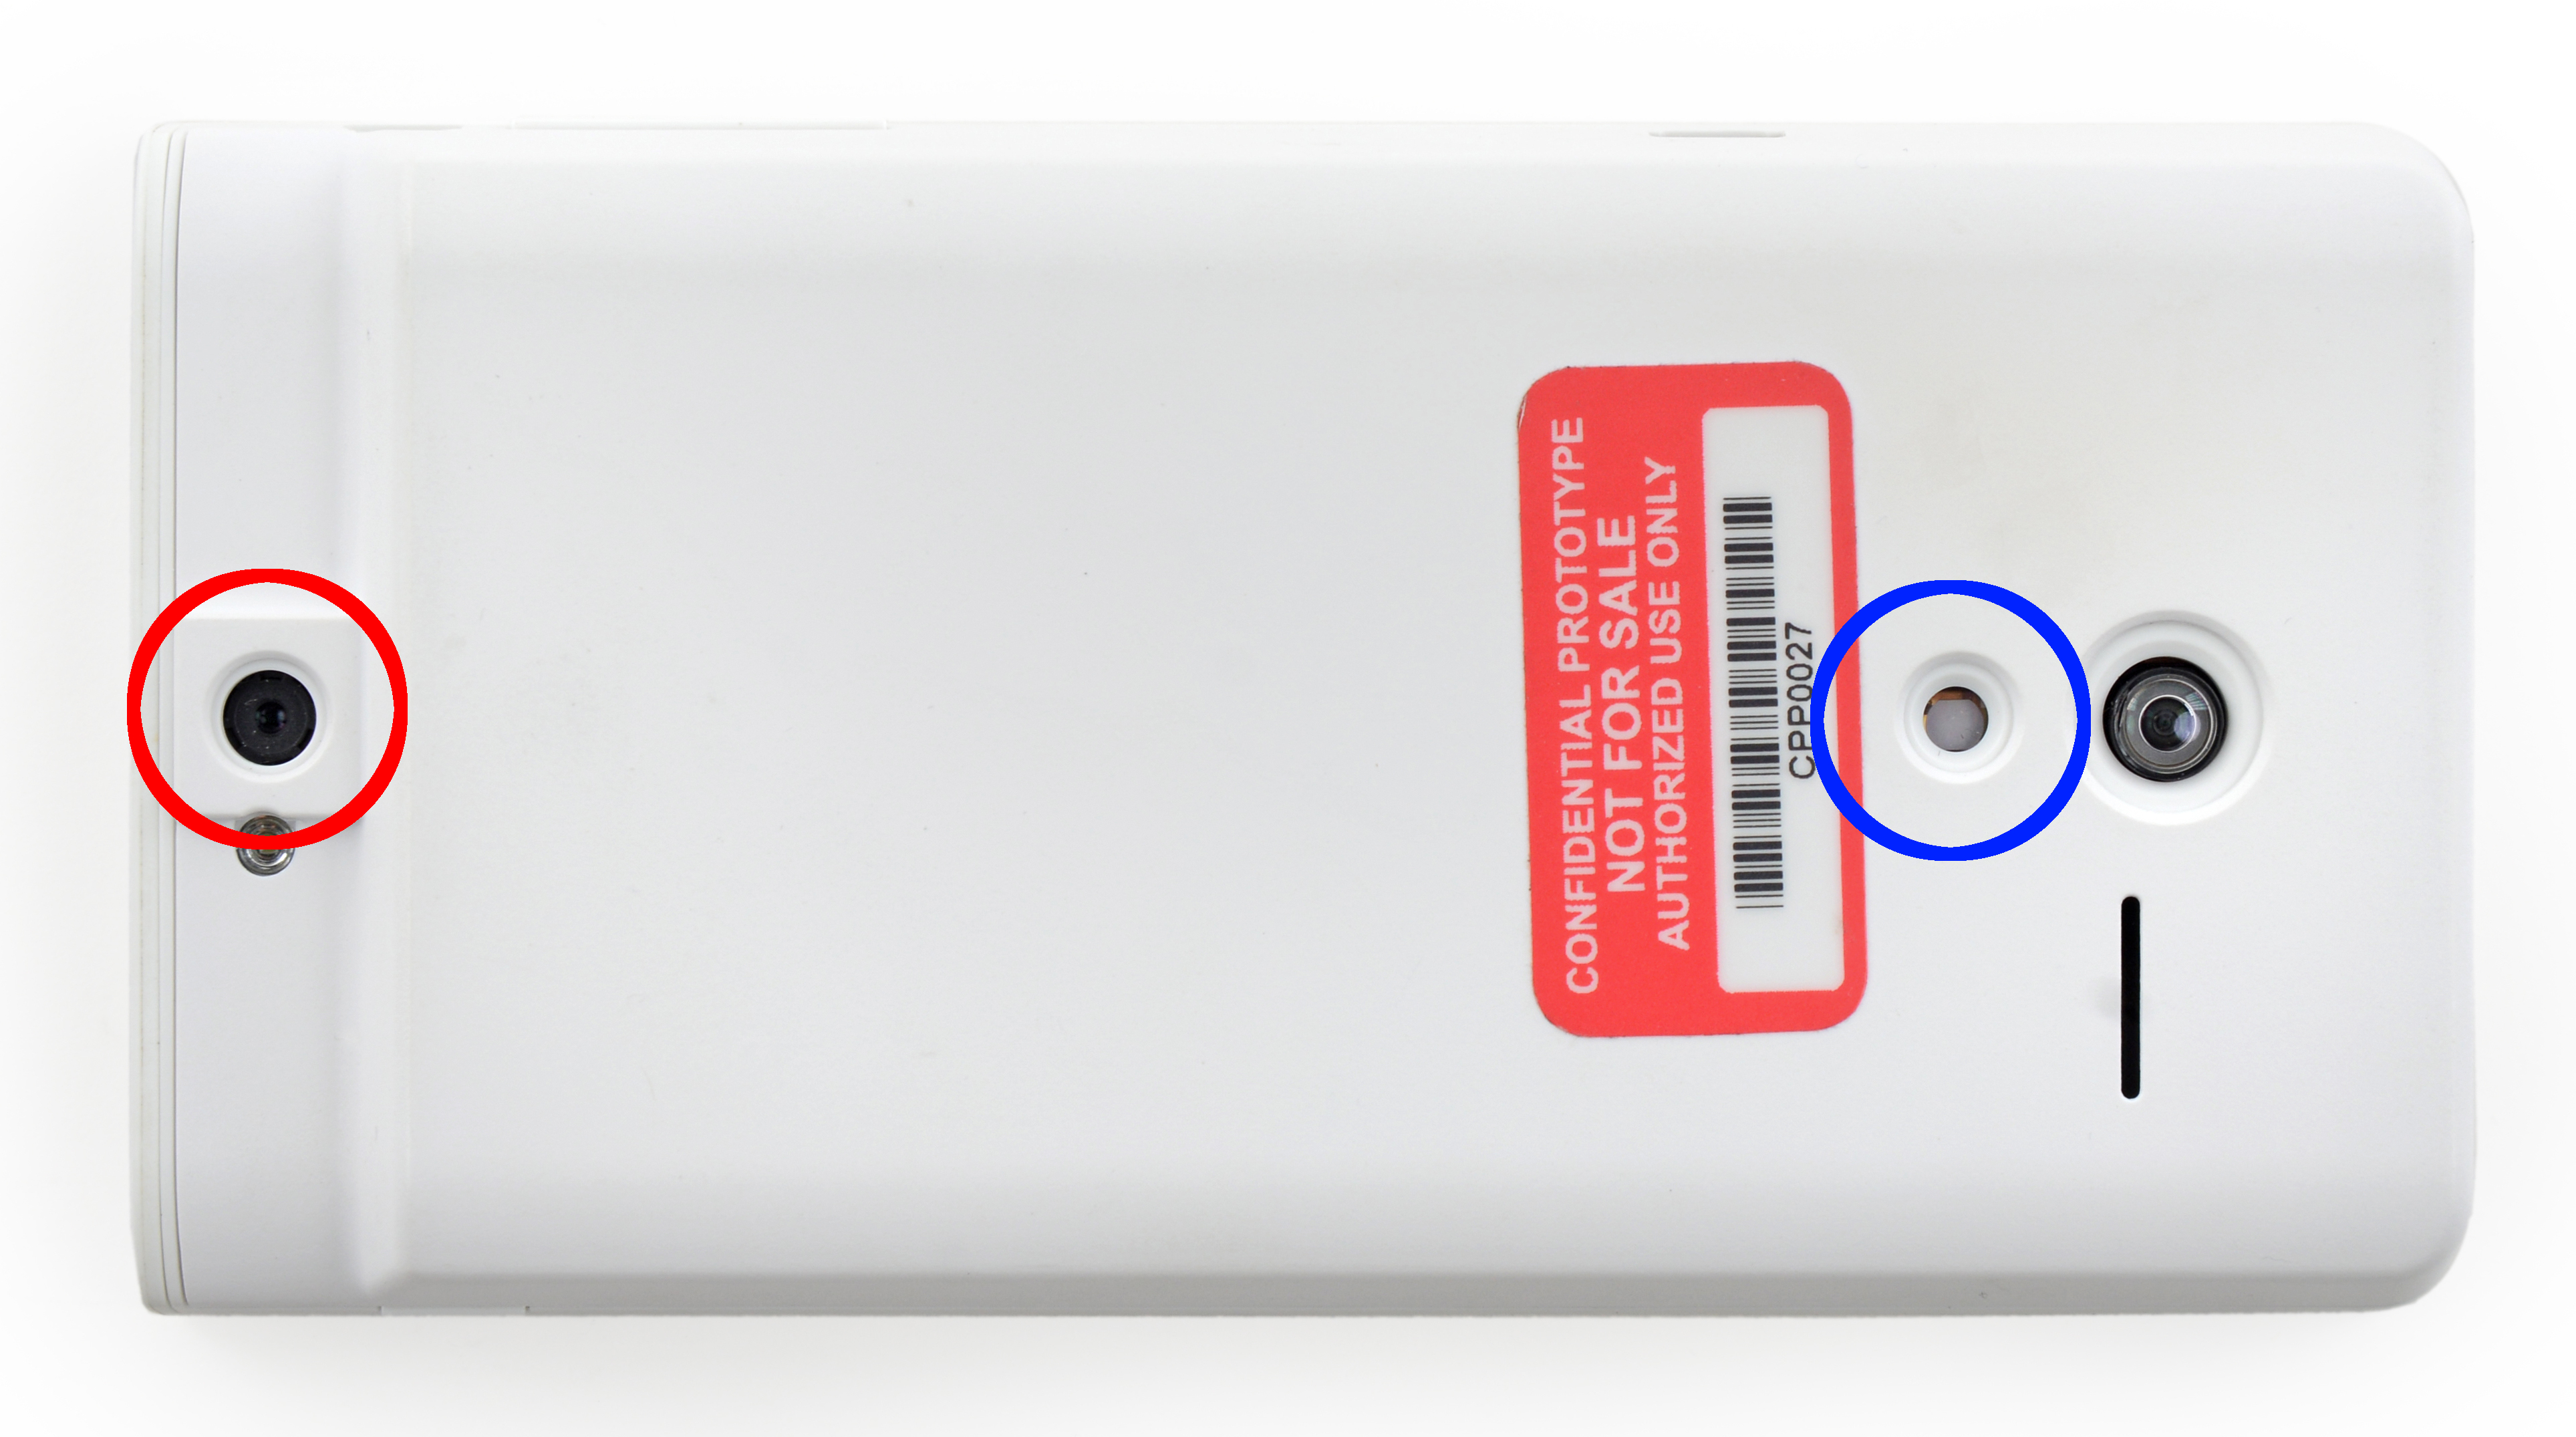
\includegraphics[scale=0.1]{TangoPhone.jpeg}
  \caption{\label{fig:tangophone} Project Tango Phone: IR camera on the left, IR projector on the right\protect\footnotemark}
\end{figure}
\footnotetext{Photo CC BY-NC-SA 3.0 by iFixit}

\begin{figure}[!h]
  \centering
  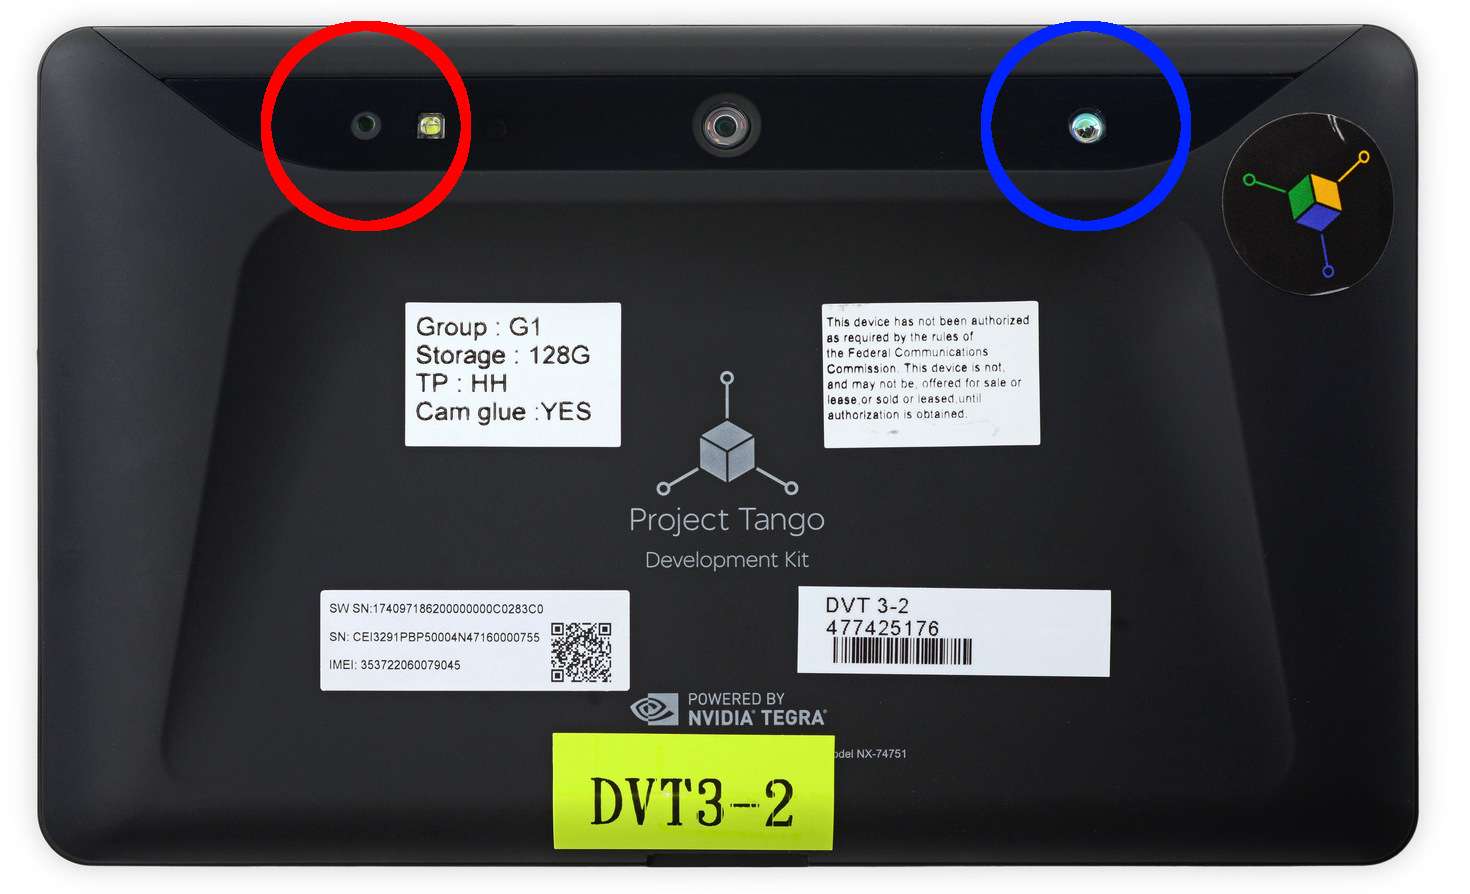
\includegraphics[scale=0.27]{TangoTab.jpeg}
  \caption{\label{fig:tangotablet} Project Tango Tablet: IR camera on the left, IR projector on the right\protect\footnotemark}
\end{figure}
\footnotetext{Photo CC BY-NC-SA 3.0 by iFixit}

We can see that the sensors are now very small and yet provides -- according to Google -- the same capabilities as the Kinect sensor. This integration of the sensors shows that our prototype could be greatly improved by using this new components.

\subsubsection{Screen resolution}
The Oculus Development team is well aware of the screen door effect and the new development kit addresses these concerns. The new Rift has a resolution of $1920\times 1080$ with a pixel density of 386ppi, whereas the first development kit had a screen resolution of $1280\times 800$ with a pixel density of 216ppi. The consummer version is expected to have a greater pixel density than the second development kit. The rising pixel density will counter the screen-door effect and allow a better representation of the surrounding scene.

\begin{figure}[!h]
  \centering
  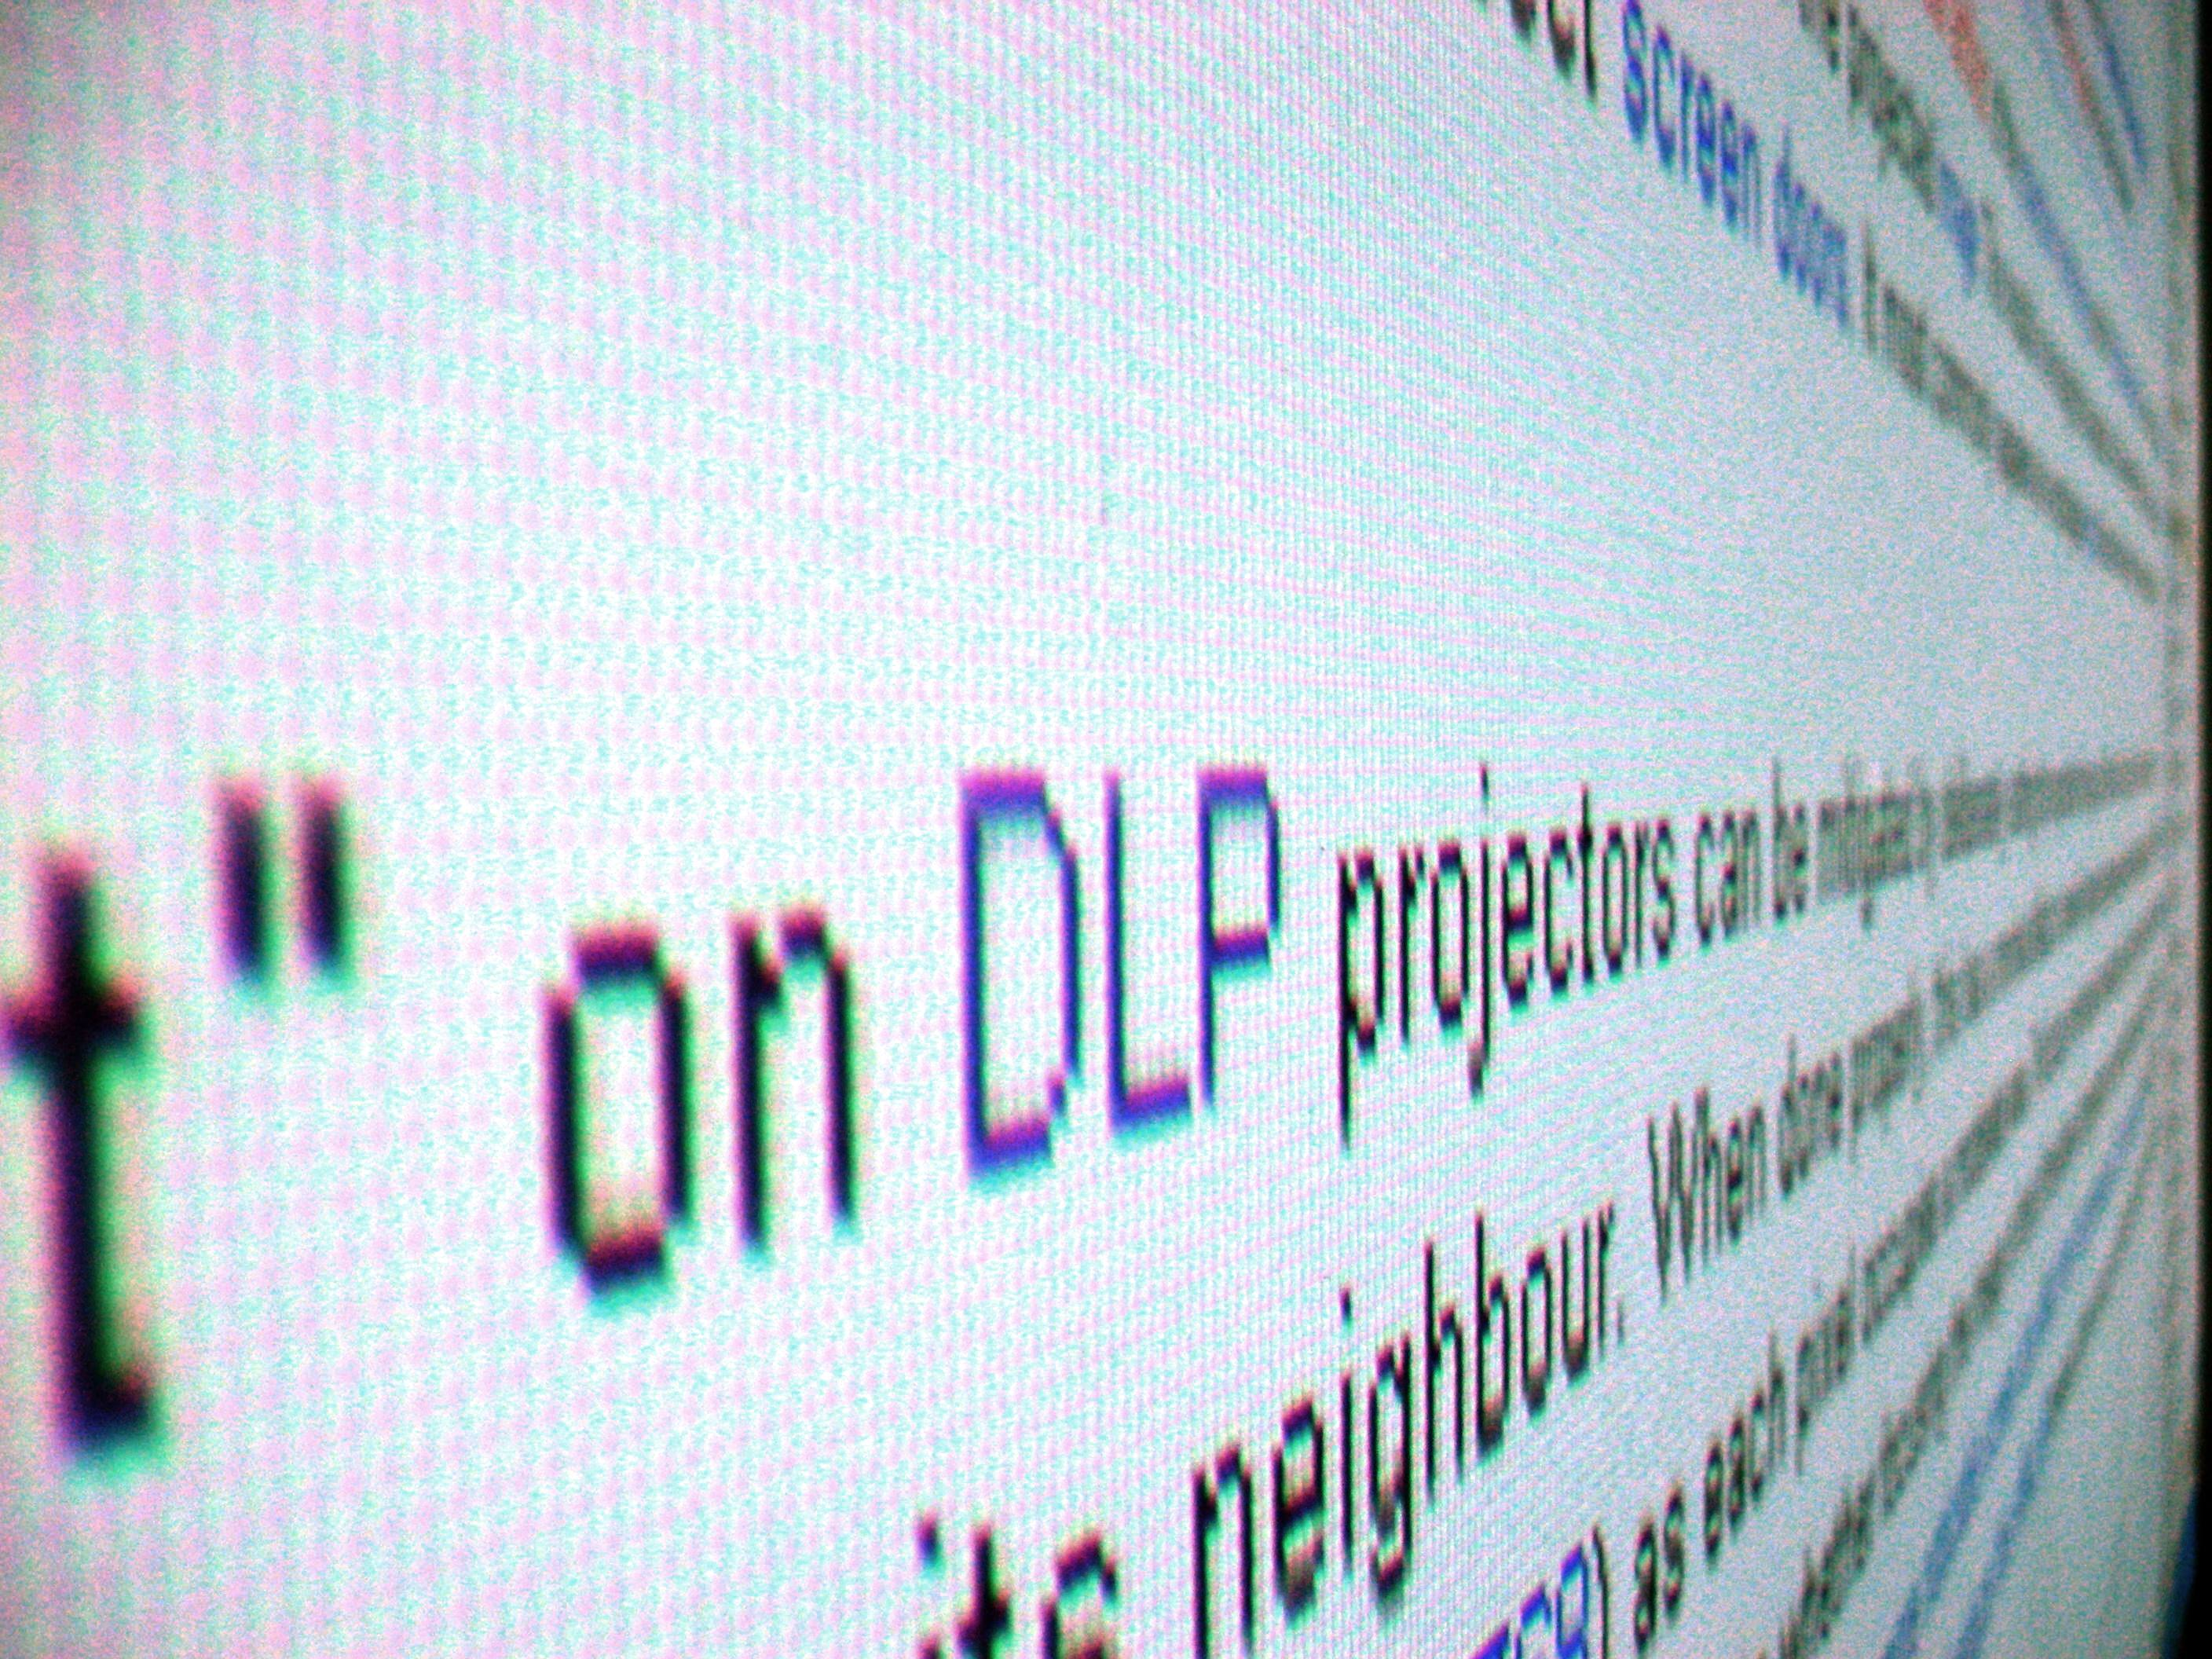
\includegraphics[scale=0.1]{Screen-door_effect.jpg}
  \caption{\label{fig:sdeffect} The screen-door effect}
\end{figure}

But in the same time, a higher screen resolution means a higher number of raycasting operations for rendering the scene. This means we need more computational power for such a scene.

\subsubsection{Computational ressources}
For our implementation, we use a GTX 780 GPU with 2304 CUDA cores. If we want to have a portable prototype, the best mobile GPU is the GTX 880M which have 1536 CUDA cores. Currently, the Project Tango uses a Tegra K1 with 192 CUDA cores. The Tegra K1 might be not powerful enough to run our implementation in real-time.

With a higher screen resolution compared to the first development kit, we need to raycast more pixels and thus we need a good GPU. While it should not be a problem for a desktop prototype like the one we built, it seems difficult to achieve a real-time headtracking, mapping and raycasting with only a Tegra K1.

\newpage
\section*{Conclusion}
\addcontentsline{toc}{section}{Conclusion}
The combination of Kinect and Oculus Rift we proposed is working almost perfectly. The device, even if is is uncomfortable, is usable and provides a strong proof of concept for the future of augmented reality devices. The user is capable of moving in the scene without stumbling around: the live color projection allows a better immersion into the 3D scene and prevents the awkward feeling of being somewhere else. The range of the reconstruction is acceptable -- a $5m^3$ box -- with a good resolution -- details such as space between keyboard keys are noticeable.

The augmented reality application \textit{Magical Pen} is simple but demonstrates the feasibility of AR applications with the device. It doesn't impact the reconstruction rate or the framerate of the rendering, making it transparent to the user. The large field of view covered by the Virtual Reality Headset suggests that Google Glass-like applications are easily transposable to our device. The coverage of the whole field of view will allow more natural integration of interaction between the user and the device.

The interest in Virtual Reality and Augmented Reality is still growing, with companies like Facebook, Apple or Google being highly interested in these fields. The Project Tango devices are almost consummer-ready smartphones and tablets capable of capturing a scene and interacting with it. It is likely to see in the next decade an improved version of our prototype for industrial or professional purpose.


\newpage
\bibliographystyle{plain}
\bibliography{biblio}
\addcontentsline{toc}{section}{References}
\end{document}